\documentclass[reprint,amsmath,amssymb,aps]{revtex4-1}

\usepackage{graphicx}
\usepackage{natbib}
\usepackage{amsmath}
\usepackage{gensymb}
\usepackage{enumerate}
\usepackage{varwidth}
\usepackage{float}
\usepackage{nonfloat}
% \usepackage{afterpage}
\usepackage[usenames, dvipsnames]{color}
\newcommand{\note}[1]{\noindent \textbf{\textit{\textcolor{Red}{#1}}}}

\newcommand\Ra{\mathrm{Ra}}
\newcommand\Pran{\mathrm{Pr}}
\newcommand\Rac{\mathrm{Ra}_{\mathrm{c}}}
\newcommand\Ek{\mathrm{Ek}}
\newcommand\Ro{\mathrm{Ro}}
\newcommand\Nu{\mathrm{Nu}}
\newcommand\Sc{\mathrm{Sc}}

\newcommand\eps{\varepsilon}
\renewcommand\L {\mathcal{L}}

\newcommand{\n}{\\ \nonumber \\ }
\newcommand{\nn}{\nonumber}
\newcommand{\nnn}{\\ \nonumber \\ \nonumber}

\newcommand\ie{\textit{i.e.},~}
\newcommand\eg{\textit{e.g.},~}
\newcommand{\omicron}{o}

\newcommand{\pd}[1]{\partial_{#1}}
\renewcommand{\vec}[1]{\boldsymbol{#1}}
\newcommand{\M}[1]{\mathbf{#1}}
\newcommand{\grad}{\vec{\nabla}}
\newcommand{\cross}{\vec{\times}}
\newcommand{\laplacian}{\nabla^2}

\newcommand{\sump}[2]{\sideset{}{'}\sum_{{#1}=0}^{#2}}

\newcommand{\eq}[1]{eq.~(\ref{#1})}
\newcommand{\eqs}[2]{eqs.~(\ref{#1})~\&~(\ref{#2})}
\newcommand{\eqss}[2]{eqs.~(\ref{#1})--(\ref{#2})}

\newcommand{\Eq}[1]{Eq.~(\ref{#1})}
\newcommand{\Eqs}[2]{Eqs.~(\ref{#1})~\&~(\ref{#2})}
\newcommand{\Eqss}[2]{Eqs.~(\ref{#1})--(\ref{#2})}

\newcommand{\fig}[1]{Fig.~(\ref{#1})}
\newcommand{\figs}[2]{Figs.~(\ref{#1})~\&~(\ref{#2})}
\newcommand{\T}{{\cal T}}
\newcommand{\Z}{{\cal Z}}

\bibliographystyle{apsrev4-1}

\makeatletter
\let\Hy@backout\@gobble
\makeatother

\newcommand*{\GtrSim}{\smallrel\gtrsim}

\makeatletter
\newcommand*{\smallrel}[2][.8]{%
  \mathrel{\mathpalette{\smallrel@{#1}}{#2}}%
}
\newcommand*{\smallrel@}[3]{%
  % #1: scale factor
  % #2: math style
  % #3: symbol
  \sbox0{$#2\vcenter{}$}%
  \dimen@=\ht0 %
  \raise\dimen@\hbox{%
    \scalebox{#1}{%
      \raise-\dimen@\hbox{$#2#3\m@th$}%
    }%
  }%
}
\makeatother


\begin{document}

\title{Marginally-Stable Thermal Equilibria of Rayleigh-Bénard Convection}

\author{Liam O'Connor$^1$}
\author{Daniel Lecoanet$^{1, 2}$}
\author{Evan Anders$^2$}
\affiliation{%
$^1$Department of Engineering Sciences and Applied Mathematics, Northwestern University, Evanston, IL 60208 USA}
\affiliation{%
$^2$Center for Interdisciplinary Exploration and Research in Astrophysics, Northwestern University, Evanston, IL, 60201 USA}

\begin{abstract}
Natural convection is ubiquitous throughout the physical sciences and engineering, yet many of its important properties remain elusive---particularly in the large Rayleigh number regime.
In this investigation, we derive and solve a quasilinear form of the Rayleigh-Benard problem by representing the perturbations in terms of marginally stable eigenmodes.
The amplitude of each eigenmode is determined by requiring that the background state maintains marginal stability.
The background temperature profile evolves due to the advective flux of each eigenmode, as well as diffusion.
The entire calculation is one-dimensional, and can be run on a workstation.
We find the background temperature field evolves to an equilibrium state, where the advective flux from the marginally-stable eigenmodes and the diffusive flux sum to a constant.
These marginally-stable thermal equilibria are exact solutions of the quasilinear equations.
The mean temperature profile has thinner boundary layers and larger Nusselt numbers than thermally-equilibrated 2D and 3D simulations of the full nonlinear equations.
We find the Nusselt number scales like $\Nu \sim Ra^{1/3}$.
When initializing a 2D simulation with a marginally-stable thermal equilibrium, we find the simulation does not exhibit the initial burst of turbulence typical of simulations initialized with the conductive background state plus noise.
Although the $\Nu$ quickly equilibrates in these simulations, the kinetic energy evolves on a viscous timescale as domain-filling flywheel flows viscously attenuate.
\end{abstract}


\maketitle

\section{Introduction}
Rayleigh-B\'enard convection plays a foundational role in large-scale astrophysical and geophysical settings.
Buoyancy-driven convection regulates heat transfer and often gives way to violently turbulent flows, thereby dominating large-scale behaviors and generating small-scale processes in important systems \cite{Couston}.

Aggressive convection, which is associated with large Rayleigh numbers $Ra$, is difficult to simulate. 
State of the art simulations performed by \cite{Zhu_2018} have reached $Ra \sim 10^{14}$ but estimates for stars are $Ra \sim 10^{20}$ \cite{Ossendrijver}. 
The scaling behavior of the Nusselt number $\Nu \sim Ra^{\beta}$ in the asymptotic ultimate regime is of particular interest.
There exists a substantial body of work pertaining to this specific topic with no general consensus \cite{Malkus_1954, Howard_1966, Kraichnan, Spiegel, Castaing, Grossman, Ahlers}. 

Reduced models are particularly useful in this context because they allow us to study the problem with relatively low expense. 
Much of the published work on this topic relates to unstable exact coherent states (ECS) \cite{Waleffe, Sondak, Wen, chini_cells}. 
Simulations and analysis performed by \cite{Yalniz, Cvitanovic} suggest that chaotic simulation trajectories can be represented by a Markov chain whose long-term behavior is given by the time-weighted-average of a finite set of unstable equilibria. Should that be the case, it is crucial that we discover and classify such equilibria.

In \cite{Beaume_2015}, researchers compute ECS in parallel shear flows by deriving and solving a quasilinear formulation of the Navier-Stokes equations via multi-scale asymptotic arguments. 
This is realized by defining a mean state which, hypothetically, evolves on a slow time-scale. 
Marginal stability is required at each successive timestep to constrain the perturbation amplitudes. 
A similar strategy is employed by \cite{michel_chini_2019}, where an analytic expression for the first-order perturbations' amplitude is found by deriving a solvability condition of the second-order perturbations and integrating over the domain spatially. 
We seek to solve the Boussinesq Rayleigh–Bénard convection equations using an analogous strategy. 
The application of this procedure yields time-invariant solutions to the quasilinear problem with a range of expected and unexpected features. 

\section{Model Setup}\label{sec:model}
We begin with the non-dimensionalized Boussinesq approximation for Rayleigh-Bénard Convection. 
The domain $\mathcal{D}$ is 2-dimensional rectangular and horizontally periodic with spatial dimensions $0 < x < 4$ and $-1/2 < z < 1/2$. 
The fluid of interest is constrained between two flat boundaries at $z = -1/2$ and $z = 1/2$ with fixed temperatures $1$ and $0$ respectively. 
At both boundaries we specify impenetrable, no-slip conditions, such that the velocity $\mathbf{u} = u \hat{x} + w \hat{z} = \mathbf{0}$ at $z = \pm 1/2$. 
The equations of motion are then given by
\begin{align}
    \nabla \cdot \mathbf{u} &= 0 \label{EQ:motion1}\\
    \frac{\partial \mathbf{u}}{\partial t} + \mathbf{u} \cdot \nabla \mathbf{u} &= - \nabla p + T \hat{z} + \mathcal{R} \nabla^2 \mathbf{u} \label{EQ:motion2}\\
    \frac{\partial T}{\partial t} + \mathbf{u} \cdot \nabla T &= \mathcal{P} \nabla^2 T \label{EQ:motion3}
\end{align}
where $p$ is pressure and $T$ is temperature. 
For completeness, we specify a final boundary condition $p = p_0$ at $z = \pm 1/2$. 
Any system of this form can be characterized by its dimensionless Rayleigh number $Ra = \frac{g\alpha L^3 \Delta T}{\nu \kappa}$ and Prandtl number $Pr = \frac{\nu}{\kappa}$, where $g, \, \alpha, \, L, \, \Delta T, \nu, \kappa$ are the gravitational acceleration, coefficient of thermal expansion, domain height, opposed temperature difference, kinematic viscosity, and thermal diffusivity respectively. For convenience, we define
\begin{equation}
\mathcal{R} = \sqrt{\frac{Pr}{Ra}}, \qquad \mathcal{P} = \frac{1}{\sqrt{Pr Ra}}.
\end{equation}

To derive the quasilinear form, we posit that an arbitrary field $f$ can be represented as the sum of a mean profile (denoted by $\bar{f}$) and a perturbation function (denoted by $f'$).
\begin{align}
    \mathbf{u}(x, z, t) &= A(t) \mathbf{u'}(x, z, t) \label{EQ:reynolds_dc_u}\\
    &= A(t) u'(x, z, t)\hat{x} + A(t) w'(x, z, t)\hat{z} \\
    T(x, z, t) &= \bar{T}(z, t) + A(t) T'(x, z, t) \label{EQ:reynolds_dc_T}\\
    p(x, z, t) &= \bar{p}(z, t) + A(t) p'(x, z, t) \label{EQ:reynolds_dc_p}.
\end{align}
where $A(t)$ is some unknown real amplitude and the mean-velocity components vanish due to incompressibility and symmetry. Perturbations must admit no horizontal-average
\begin{equation}
    \langle f'(x, z, t) \rangle_x \equiv \int_{0}^4 f'(x, z, t) dx = 0.
\end{equation}
Assuming the existance of nontrivial solutions, we also fix the volume-average over the entire domain
\begin{equation}
  \langle T'^2 \rangle_{\mathcal{D}} = 1
\end{equation}
thereby alleviating any ambiguity in $A(t)$. 
Substituting (\ref{EQ:reynolds_dc_T}) into (\ref{EQ:motion3}) and taking the horizontal-average reduces the system to a simple initial value problem (IVP) for $\bar{T}$
\begin{equation}
  \frac{\partial \bar{T}}{\partial t} + A^2 \langle w'T' \rangle_x = \mathcal{P}  \frac{\partial^2 \bar{T}}{\partial z^2}, \label{EQ:T0_IVP}
\end{equation}
with associated boundary conditions $\bar{T}(-1/2, t) = 1$ and $\bar{T}(1/2, t) = 0$. It should be noted that we could obtain a similar IVP for $u$ by breaking symmetry and considering some nontrivial mean horizontal flow $\bar{u}(z, t)$. However we must have $\bar{w}(z, t) = 0$ due to incompressibility.

To solve (\ref{EQ:T0_IVP}) numerically, we need the perturbations and their associated amplitude function $A(t)$. 
The former is obtained by solving the linearized system. Substituting (\ref{EQ:reynolds_dc_u})--(\ref{EQ:reynolds_dc_p}) into (\ref{EQ:motion1})--(\ref{EQ:motion3}) and subtracting (\ref{EQ:T0_IVP}) from the resulting temperature equation gives
\begin{align}
    \nabla \cdot \mathbf{u'} &= 0 \label{EQ:linear1}\\
    \frac{\partial\mathbf{u'}}{\partial t} &= - \nabla p' + T'\hat{z} + \mathcal{R} \nabla^2 \mathbf{u'} \label{EQ:linear2}\\
    \frac{\partial T'}{\partial t} + \frac{\partial \bar{T}}{\partial z} w' &= \mathcal{P} \nabla^2 T' \label{EQ:linear3}
\end{align}
with Dirichlet boundary conditions 
\begin{equation}
    T'|_{z = \pm \frac{1}{2}} = 0, \quad u'|_{z = \pm \frac{1}{2}} = 0, \quad p'|_{z = \pm \frac{1}{2}} = 0.
\end{equation}

In his groundbreaking report \cite{Rayleigh_1916}, Lord Rayleigh observed that (\ref{EQ:linear1}) and (\ref{EQ:linear3}) can be manipulated into a separable form with generalized solutions
\begin{align}
    w'(x, z, t) &= W(z) \, e^{i(k_xx-st)} \label{EQ:normal_modes1}\\ 
    u'(x, z, t) &= U(z) \, e^{i(k_xx-st)} \label{EQ:normal_modes2}\\ 
    T'(x, z, t) &= \theta(z) \, e^{i(k_xx-st)} \label{EQ:normal_modes3}\\ 
    p'(x, z, t) &= P(z) \, e^{i(k_xx-st)}\label{EQ:normal_modes4}
\end{align}
where $s = \sigma + i\omega$ and $k_x$ is constrained, by periodicity, to the countably infinite set (spectrum) of wavenumbers
\begin{align}
    k_x \in \big\{\frac{n\pi}{2} \, \big| \, n \in \mathbb{N}\big\}.
\end{align}
For each $k_x$, we can assess the stability of the perturbations by solving for the eigenvalue $s$, whose imaginary component $\omega$ plays the role of an exponential growth rate. 
Solution yields a finite set of eigenvalues, among which, that with maximum $\omega$ is assumed to be dominant. 
Positive eigenvalues indicate that the system is unstable to small disturbances of wavenumber $k_x$, while negative eigenvalues indicate stability. 
A complete linear stability analysis requires solution over the full spectrum of wavenumbers. 
The prototypical case is used to demonstrate that the critical Rayleigh number $Ra_c = 1708$ when $\frac{\partial \bar{T}}{\partial z} = -1$.
 
At some arbitrary time $t_0$, the forcing term $\langle w'T' \rangle_x$ can be found by solving an eigenvalue problem (EVP) which itself involves $\frac{\partial \bar{T}}{\partial z}$. 

\section{Perturbation Evolution}
Solving the linearized system (\ref{EQ:linear1})--(\ref{EQ:linear3}) does not yield $A(t)$. 
To evolve $\bar{T}$, we assume the perturbations and mean quantities evolve according to different time-scales, as in \cite{michel_chini_2019}.
Stable modes decay away rapidly. 
Unstable modes will not persist on the slow time-scale because the advective term $\langle w'T' \rangle_x$ tends to stabilize $\bar{T}$, thereby creating a negative feedback loop. Only marginally stable modes can traverse this hypothetical time-scale separation. Therefore the amplitude function $A(t)$ must satisfy
\begin{equation}
    \max_{k_x} \{ \omega \} = 0.
\end{equation}

For various $Ra$ and fixed $Pr = 1$, we seek symmetric marginally-stable thermal equilibria (MSTE), thereby satisfying $\frac{\partial \bar{T}}{\partial t} = 0$ according to (\ref{EQ:T0_IVP}). 
We employ the \texttt{Dedalus} pseudo-spectral python framework to solve the EVP outlined in Section \ref{sec:model} as well as the IVP (\ref{EQ:T0_IVP}) by representing each field with a dealiased Chebyshev polynomial basis. 
The necessary number of basis functions varies, as eigenfunctions and temperature profiles associated with large $Ra$ admit increasingly small-scale features. 
We supplement \texttt{Dedalus} with the \texttt{Eigentools} package to compute $\langle w' T' \rangle_x$.

At $t = 0$, we begin with a marginally-stable initial profile $\bar{T}(z, 0)$ whose construction is outlined in \ref{sec:initial_profile}. 
At some arbitrary time $t = t_0$, we seek to evolve $\bar{T}(z, t_0)$ into a new marginally-stable profile $\bar{T}(z, t_0 + \Delta t)$ according to (\ref{EQ:T0_IVP}) via forward-Euler. 
This generally involves a unique and unknown value $A^2(t_0) > 0$. 
Our method of finding $A^2(t_0)$ is best illustrated through example.

\begin{figure}
    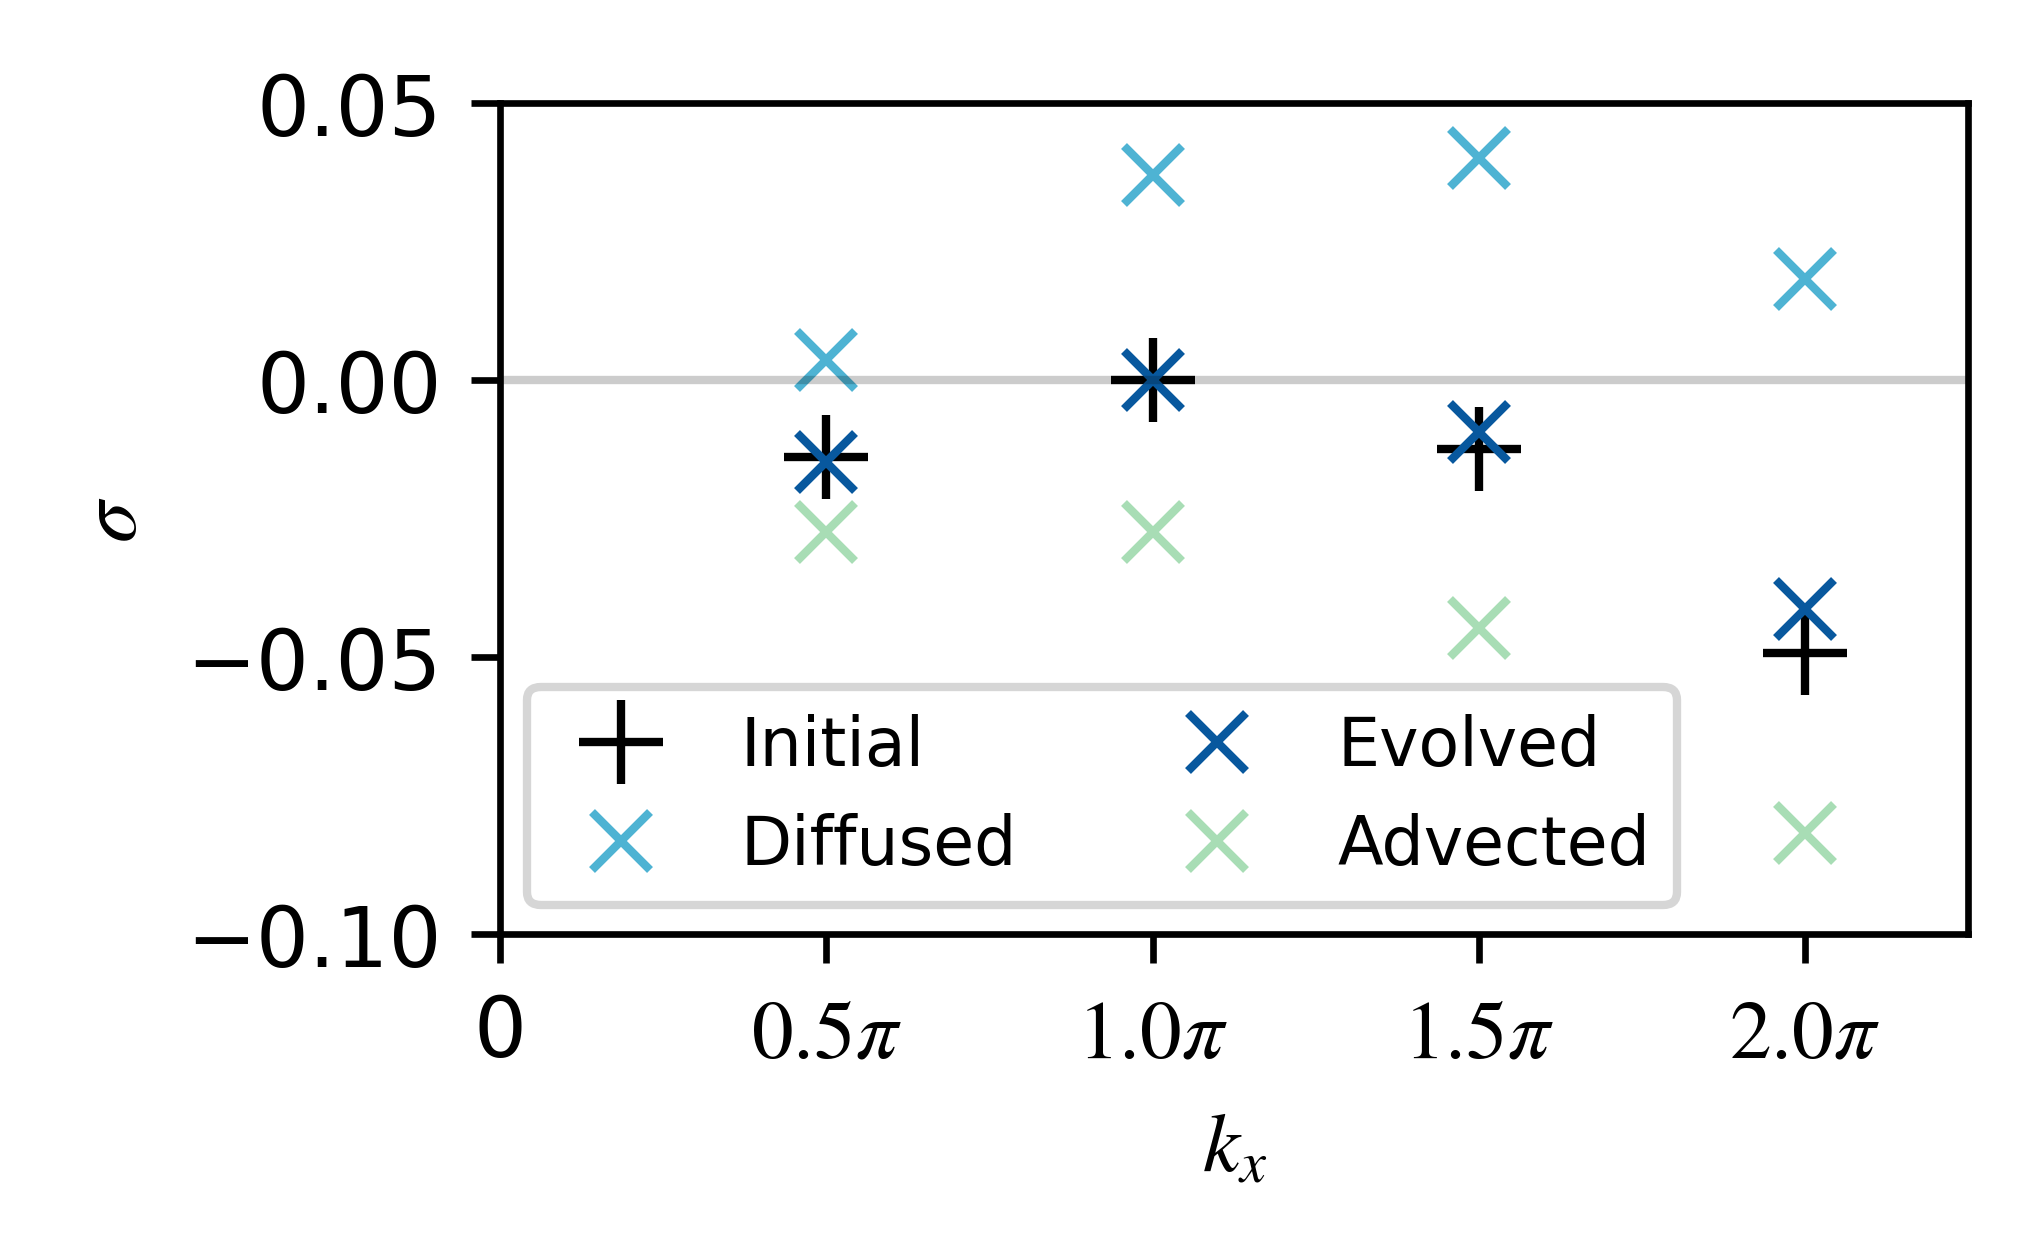
\includegraphics[width=3.4in]{EV_spectrum_ol.png}
    \caption{Eigenvalue spectra for $Ra = 10^5$. The spectrum of an ``initial" marginally-stable mean temperature profile $\bar{T}(z, t_0)$ has a maximum eigenvalue of 0. 
    Given a small fixed timestep $\Delta t$, diffusion destabilizes the system, increasing its eigenvalues. 
    Advection tends to stabilize the system, decreasing its eigenvalues. 
    It follows that there exists some proportion $A^2(t_0)$ of these two terms which yields a new marginally-stable mean temperature profile $\bar{T}(z, t_0 + \Delta t)$, whose spectrum is ``evolved".}
    \label{fig:iteration_spectra} 
\end{figure}

An iteration is performed as follows: diffusing a marginally-stable temperature profile $\bar{T}(z, t_0)$ tends to increase its eigenvalues. 
Ignoring the diffusive term and evolving according to advection tends the stabilize the system. The appropriate amplitude $A^2(t_0)$ can then be approximated by
\begin{equation}
    A^2(t_0) \sim -\frac{\omega_{\rm{diff}}}{\omega_{\rm{adv}}}
\end{equation}
where $\omega_{\rm{diff}}$ and $\omega_{\rm{adv}}$ refer to the diffused and advected eigenvalues of the initially marginal mode. These quantities correspond to the light blue and green points at $k_x = \pi$ in Figure \ref{fig:iteration_spectra}). 
$\bar{T}(z, t)$ is then evolved according to (\ref{EQ:T0_IVP}) and another eigenvalue solve is performed. 
Given a fixed timestep $\Delta t$, we assume the dominant eigenvalue can be described by a continuous function $\omega_{\rm{max}} (A^2)$ which is locally differentiable. 
We use Newton's method to find an amplitude which satisfies our marginal stability tolerance criterion. 
The dominant mode is not fixed; an iteration can facilitate the transfer of marginal-stability from one mode to another. 
In section \ref{sec:multiple_modes} we specify procedures for the treatment of multiple simultaneously marginal modes.

\subsection{Treatment of multiple marginally-stable modes} \label{sec:multiple_modes}
In most cases, we eventually encounter eigenvalue spectra with multiple simultaneously marginal modes. If ignored, we are forced to reduce the timestep and allow the modes to alternate. Instead, we generalize the advective term in (\ref{EQ:T0_IVP}) to accommodate $N$ simultaneously marginal modes
\begin{equation}
    A^2 \langle w' T' \rangle_x = \sum_{n = 1}^{N} A^2_{n} \langle w' T' \rangle_{x, \, n}
\end{equation}
where  $\langle w' T' \rangle_{x, \, n}$ is composed of perturbations associated with $k_x = \frac{n\pi}{2}$. 
There are now $N$ amplitudes to solve for and $N$ eigenvalues to keep marginally-stable. 
In general, we expect a function $\mathbf{\omega} \, : \, \mathbb{R}^N \to  \mathbb{R}^N$ to have isolated roots (should they exist). 
We employ Broyden's method for root-finding in multi-dimensional functions whose derivatives are not explicitly known. 
Difficulty arises when transitioning between different numbers of marginal modes. 
Here we rely on $A^2 > 0$ by asserting that a mode which is \textit{close enough} to marginal-stability can be included in the iteration provided that its respective amplitude is positive. 
Should we converge upon a negative amplitude, that mode is discarded and the iteration is repeated. 
In general we find that no other obvious course of action yields equilibria.

\section{Properties of Thermally Equilibrated States}\label{sec:properties}
MSTE are fixed points of the quasilinear form derived in section \ref{sec:model}, differing from ECS in that ECS are fixed points of the full nonlinear problem (\ref{EQ:motion1})--(\ref{EQ:motion3}). 
Such definitions are not mutually exclusive, but in general we can assume that MSTE and ECS are not steady with respect to their counterparts' problems.
For this investigation, we calculate solutions for $Ra$ in the range $10^5 - 10^9$. 
Their mean temperatures $\bar{T}$ are symmetric about $z = 0$ by construction. 

\begin{figure}
    \centering
    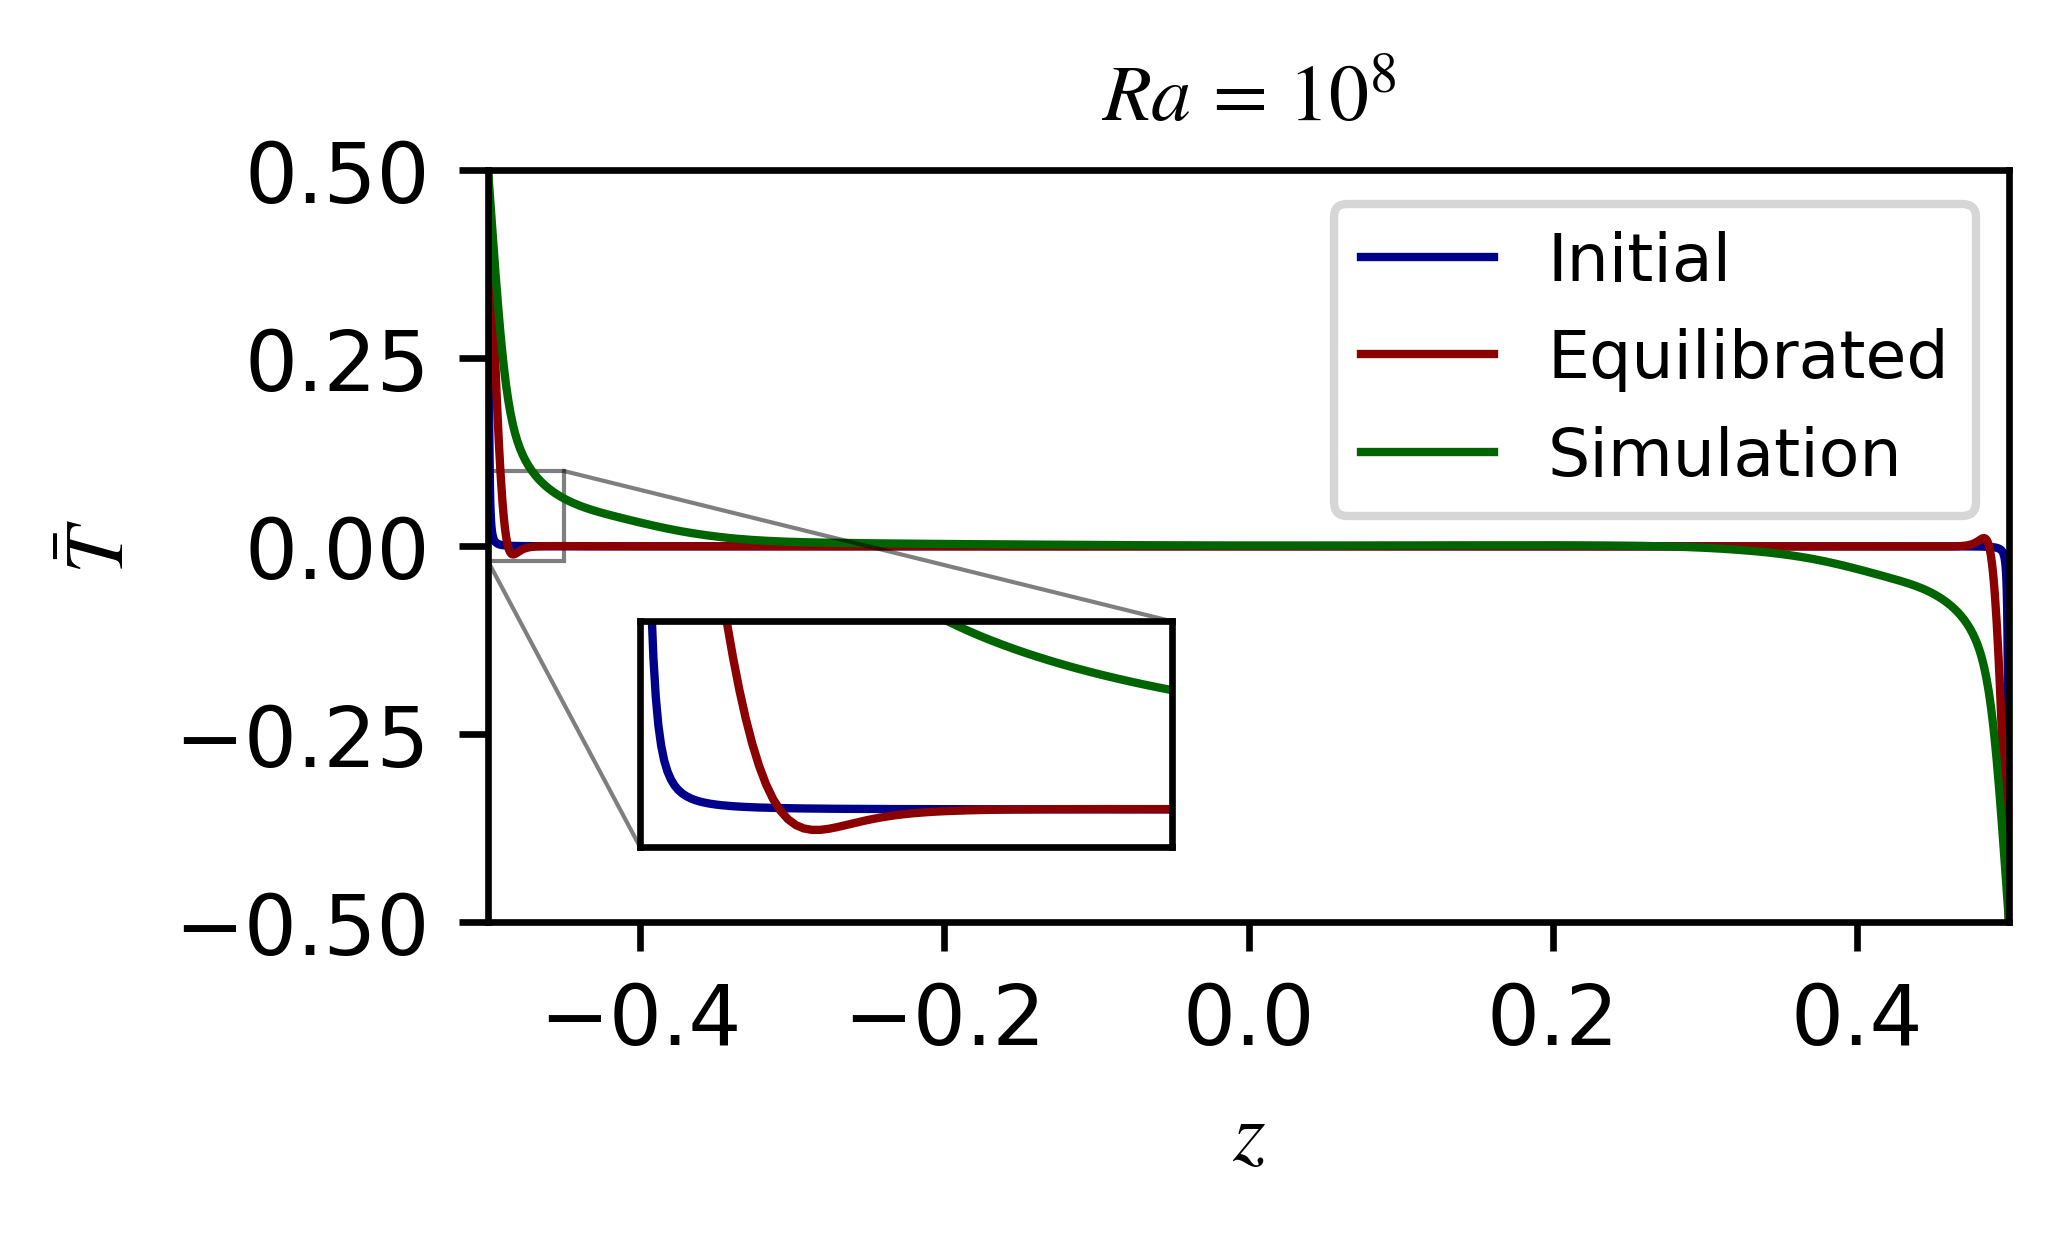
\includegraphics[width=3.4in]{T_profs_na.png}
    \caption{Mean temperature profiles $\bar{T}$ for $Ra = 10^8$. 
    The initial profile is given by (\ref{EQ:T0}). 
    The MSTE curve refers to the mean temperature profile of the marginally-stable thermally-equilibrated state. 
    The DNS profile is obtained by performing a 2-dimensional nonlinear simulation of (\ref{EQ:motion1})--(\ref{EQ:motion3}) with \texttt{Dedalus} until thermal and kinetic relaxation. 
    The DNS temperature data are horizontally- and time-averaged. 
    The initial, MSTE, and DNS profiles have increasingly relaxed boundary regions (respectively). 
    The MSTE profile exhibits prominent dips, nested alongside the boundary regions. 
    The source of this feature is not well understood, but similar temperature gradient reversal regions were found by \cite{chini_cells} along the midlines of 2-dimensional convective cellular solutions at $Ra \sim 10^6$.}
    \label{fig:T0_profiles}
\end{figure}

Figure \ref{fig:T0_profiles} gives temperature profiles for $Ra = 10^8$ where the initial profile, given by (\ref{EQ:T0}), is employed at iteration 0; the MSTE profile corresponds to the thermally relaxed state; and the DNS (direct numerical simulations) profile is obtained by solving (\ref{EQ:motion1})--(\ref{EQ:motion3}) with \texttt{Dedalus}, followed by horizontal- and time- averaging. 
The DNS curve is more diffuse than the MSTE curve, which in turn, is more diffuse than the initial curve. 
Performing an eigenvalue solve by setting $\bar{T}$ equal to the DNS profile yields positive eigenvalues. 
Comprehensively, this suggests that MSTE might maximize boundary layer thickness, while subject to the marginal stability constraint.

The most resilient and unexpected feature of MSTE temperature profiles are the pronounced dips adjacent to the boundary layers. 
These dips appear in every solution, regardless of $Ra$. 
Physically, they correspond to thin layers in which the mean temperature gradient reverses, contradicting an important hypothesis of \cite{Malkus_1954}. 
This counter-diffusion, which opposes overall heat transfer, is overcome by the coinciding advective flux, shown in Figure \ref{fig:flux}. 
We don't understand the source of these dips, but similar temperature gradient reversals were reported by \cite{chini_cells} along the midlines of 2-dimensional convective cellular solutions at $Ra \sim 10^6$. 


\begin{figure*}
    \centering
    \begin{tabular}{@{}c@{}}
        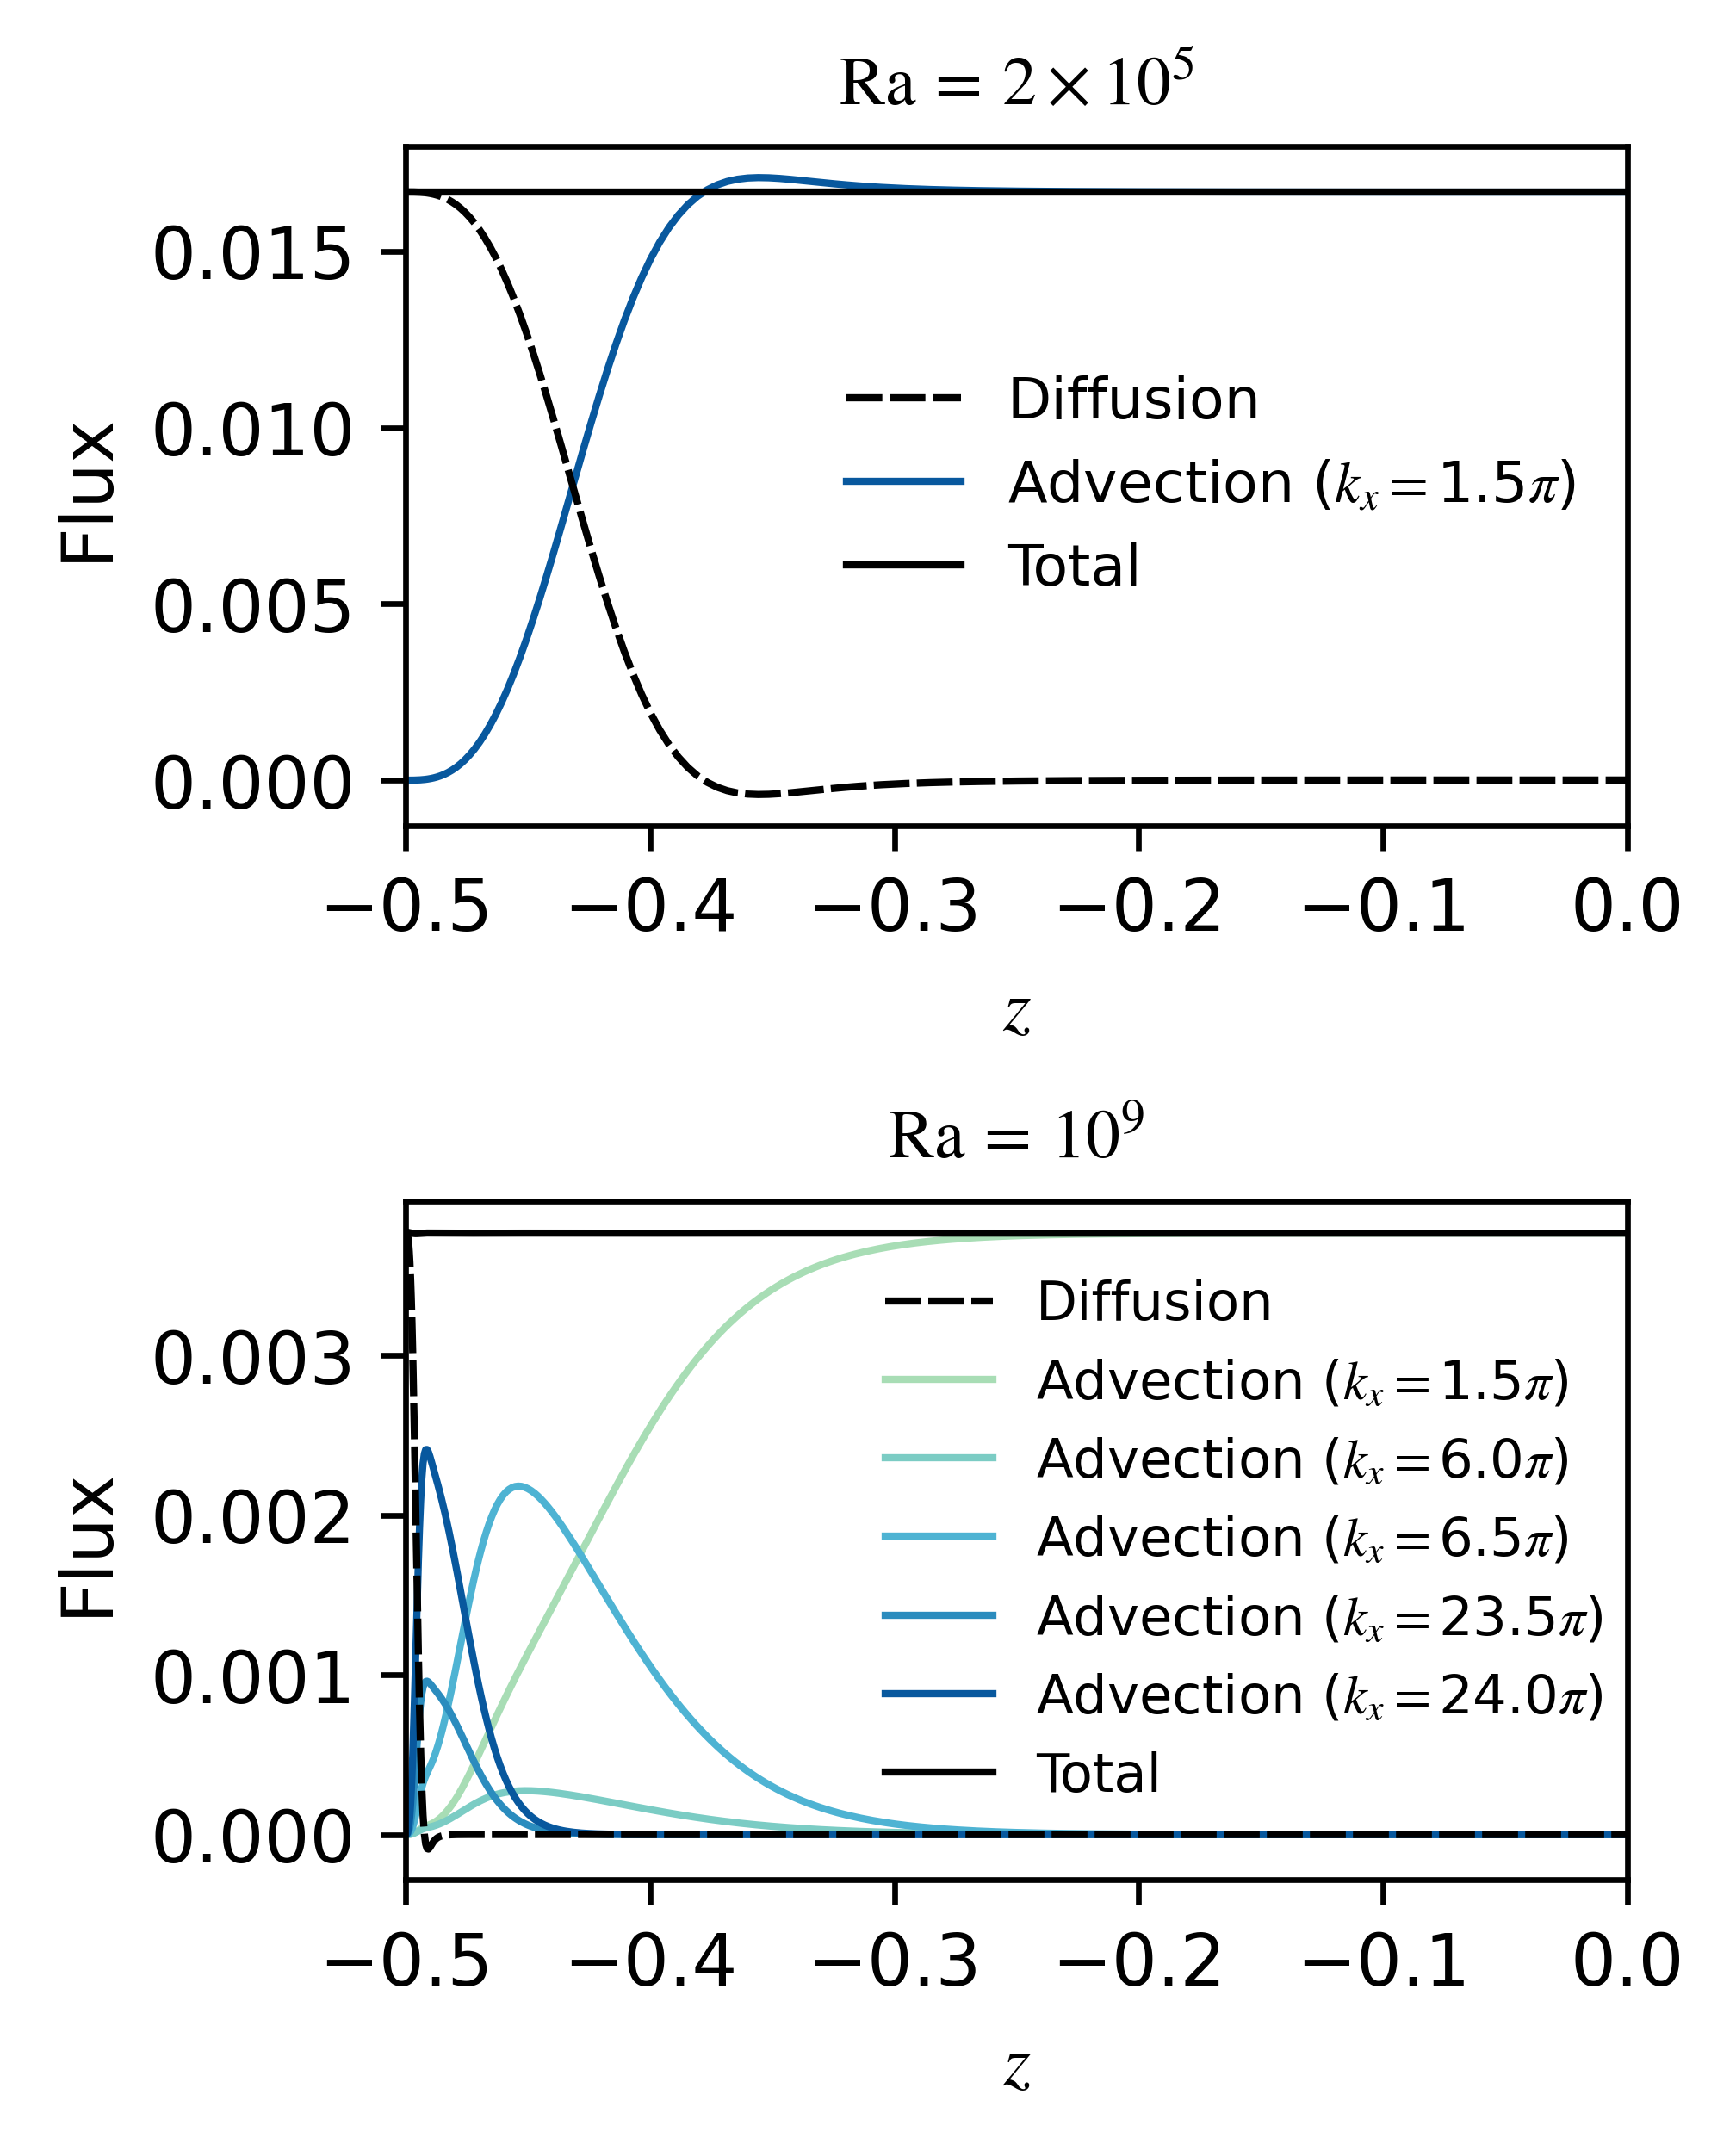
\includegraphics[width=3.4in]{flux_sup_n.png}
    \end{tabular}
    \begin{tabular}{@{}c@{}}
        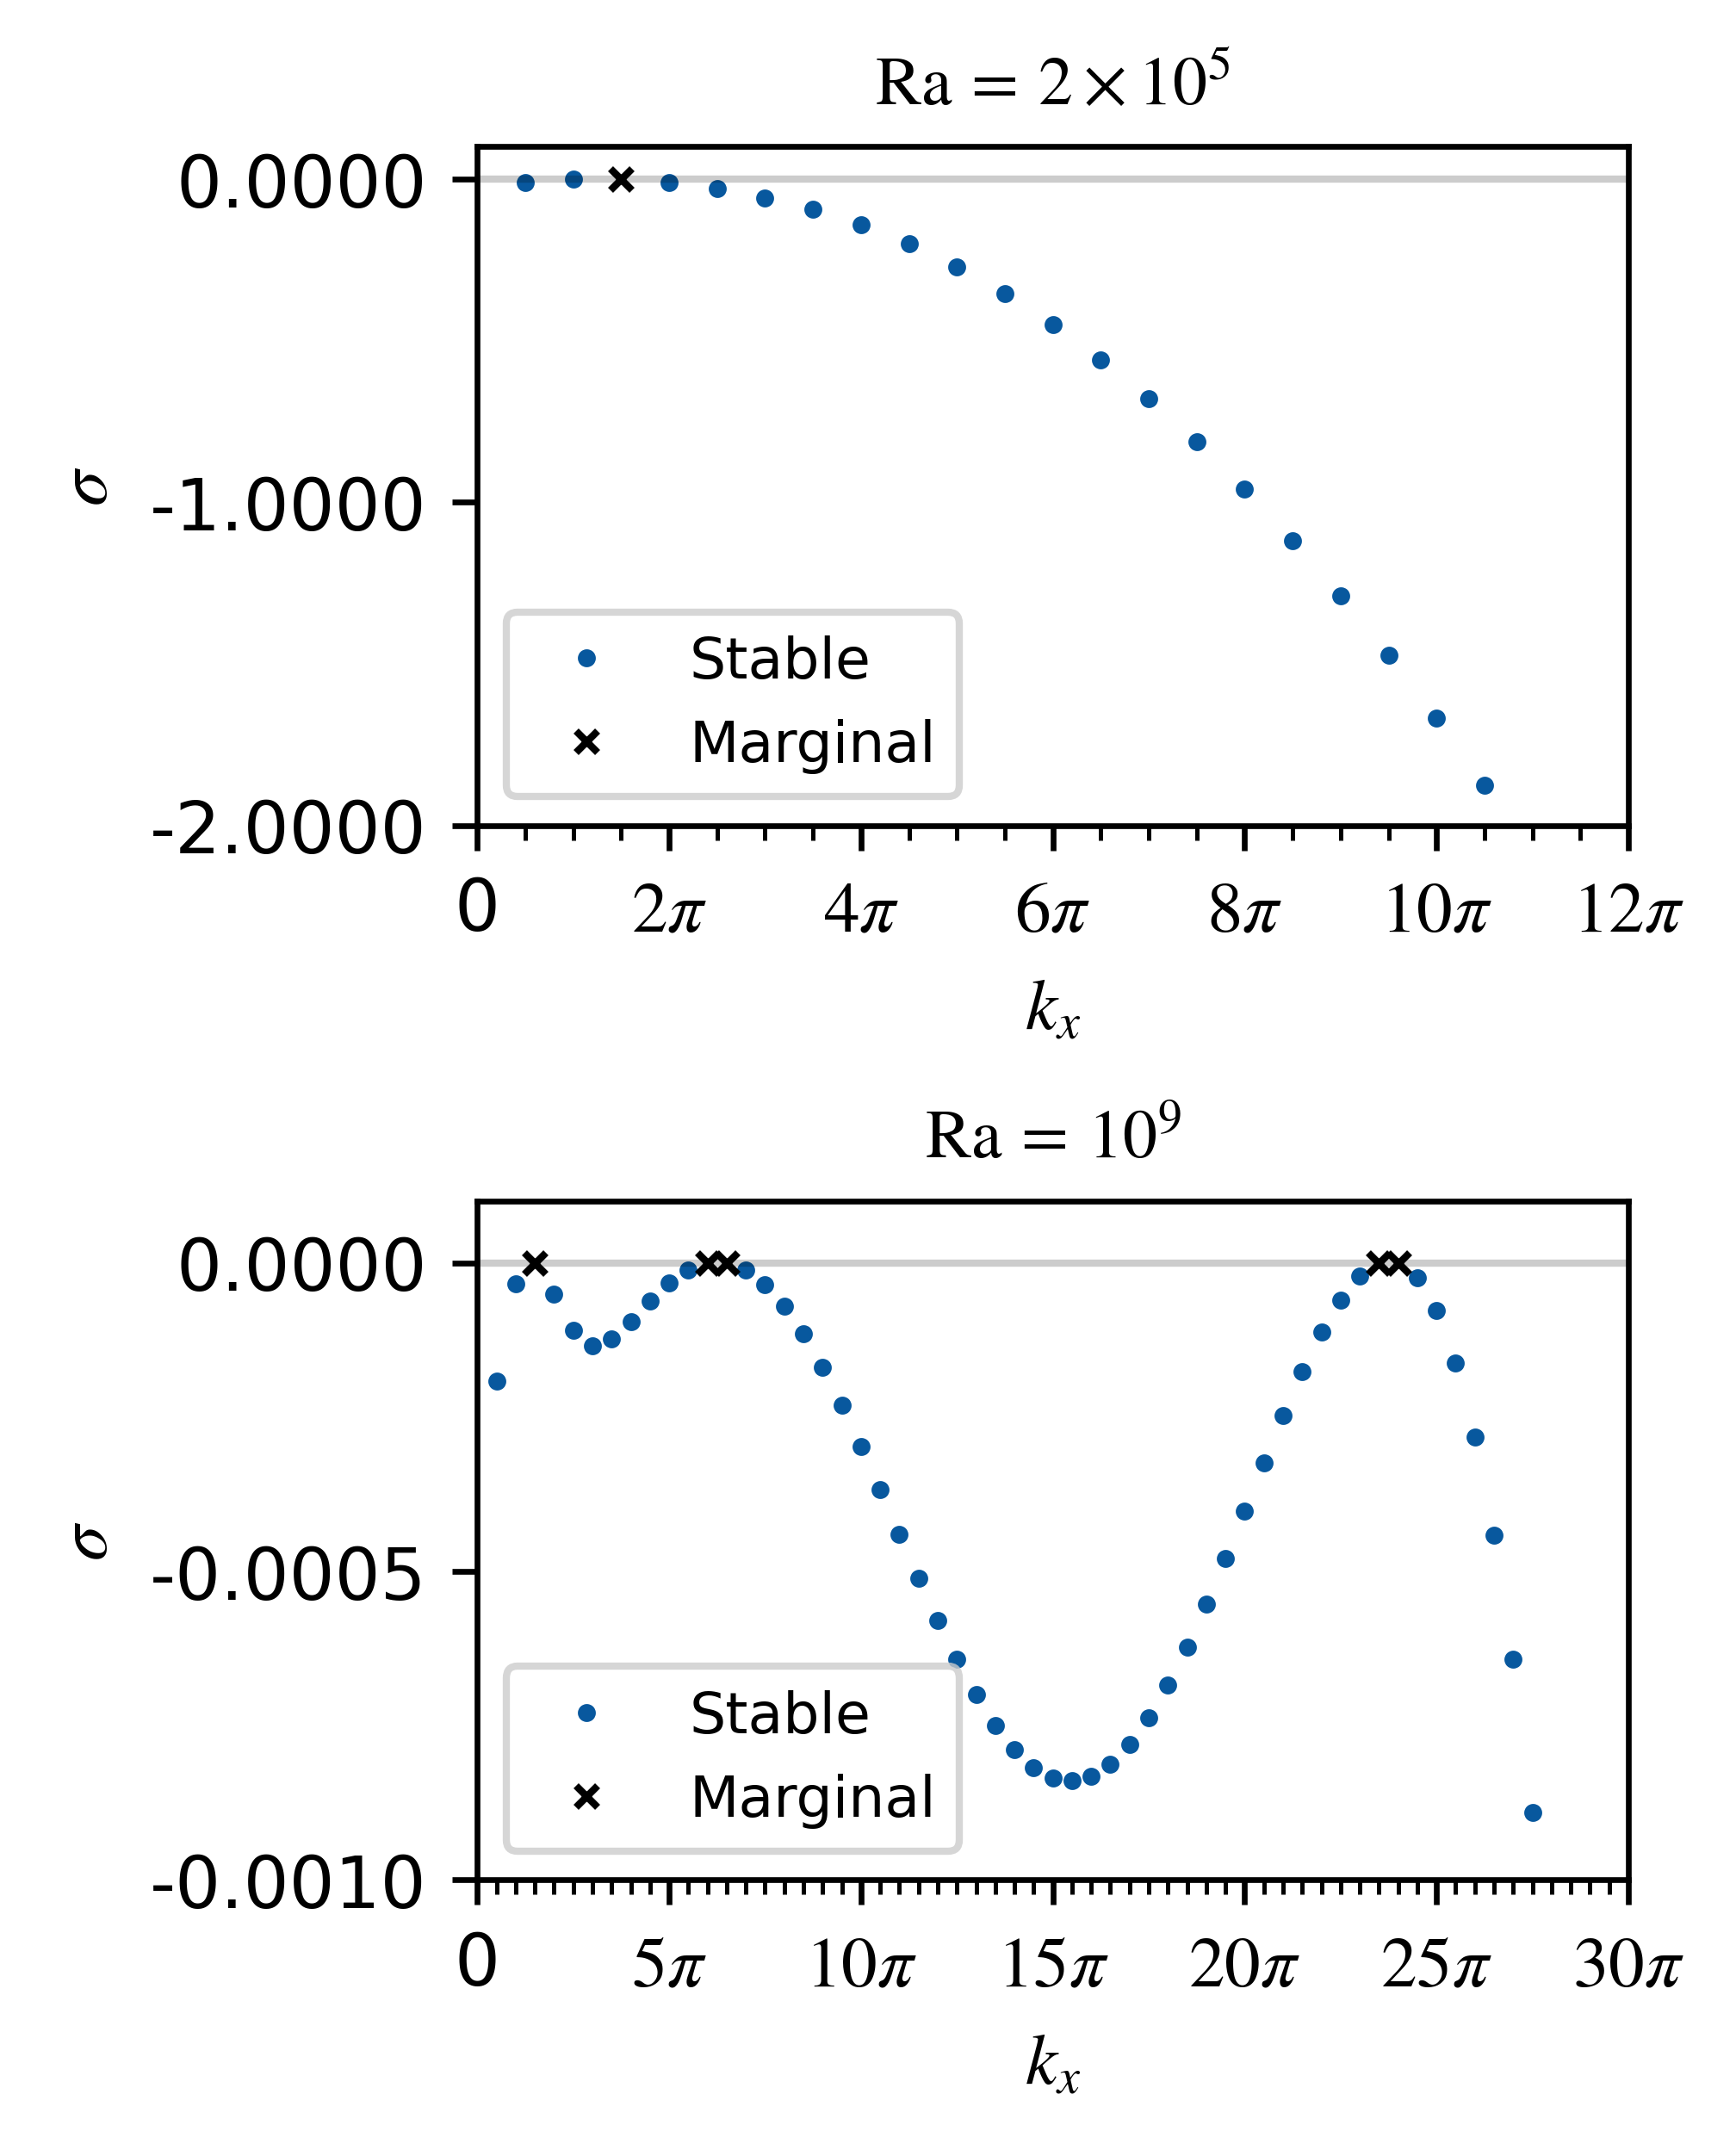
\includegraphics[width=3.4in]{EV_spectra_2ra.png}
    \end{tabular}
    \caption{Heat fluxes (left) and eigenvalue spectra (right) of equilibrated states $Ra = 2 \times 10^5$ (top) and $Ra = 10^9$ (bottom). 
    Advection profiles belong to marginally-stable modes. 
    For low $Ra$, a single mode with $k_x = 1.5\pi$ is sufficient to oppose boundary layer diffusion and facilitate heat flux throughout the bulk of the domain. 
    For large $Ra$, high-wavenumber modes contribute pronounced small-scale advection profiles which tightly hug the thin boundary layers. 
    A combination of of progressively wider advection profiles is necessary to transition to the $k_x = 1.5\pi$ mode.}
    \label{fig:flux}
\end{figure*}

Equilibrated states exhibit distinct behaviors for large and small $Ra$. 
This contrast is illustrated in Figure \ref{fig:flux}, where we give heat flux profiles and eigenvalue spectra for two cases: $Ra = 2 \times 10^5$ and $Ra = 10^9$. 
For $Ra = 2 \times 10^5$, there is a single presumed local maximum in the eigenvalue spectrum, whose adjacent modes' advection profiles occupy the bulk of the domain. 
These states have relaxed boundary layers which gradually subside as advection becomes the dominant flux component. 
Such transitional regions do not appear for $Ra = 10^9$, where the shift from diffusion to advection is sharp, requiring pronounced, small-scale advection profiles belonging to modes in the third local maxima pair of the eigenvalue spectrum. 
Traversing towards the midline of the domain, we see increasingly thicker advection profiles corresponding to modes in the second local maxima pair, eventually culminating in the dominant $k_x = 1.5\pi$ mode.

\begin{figure}
    \centering
    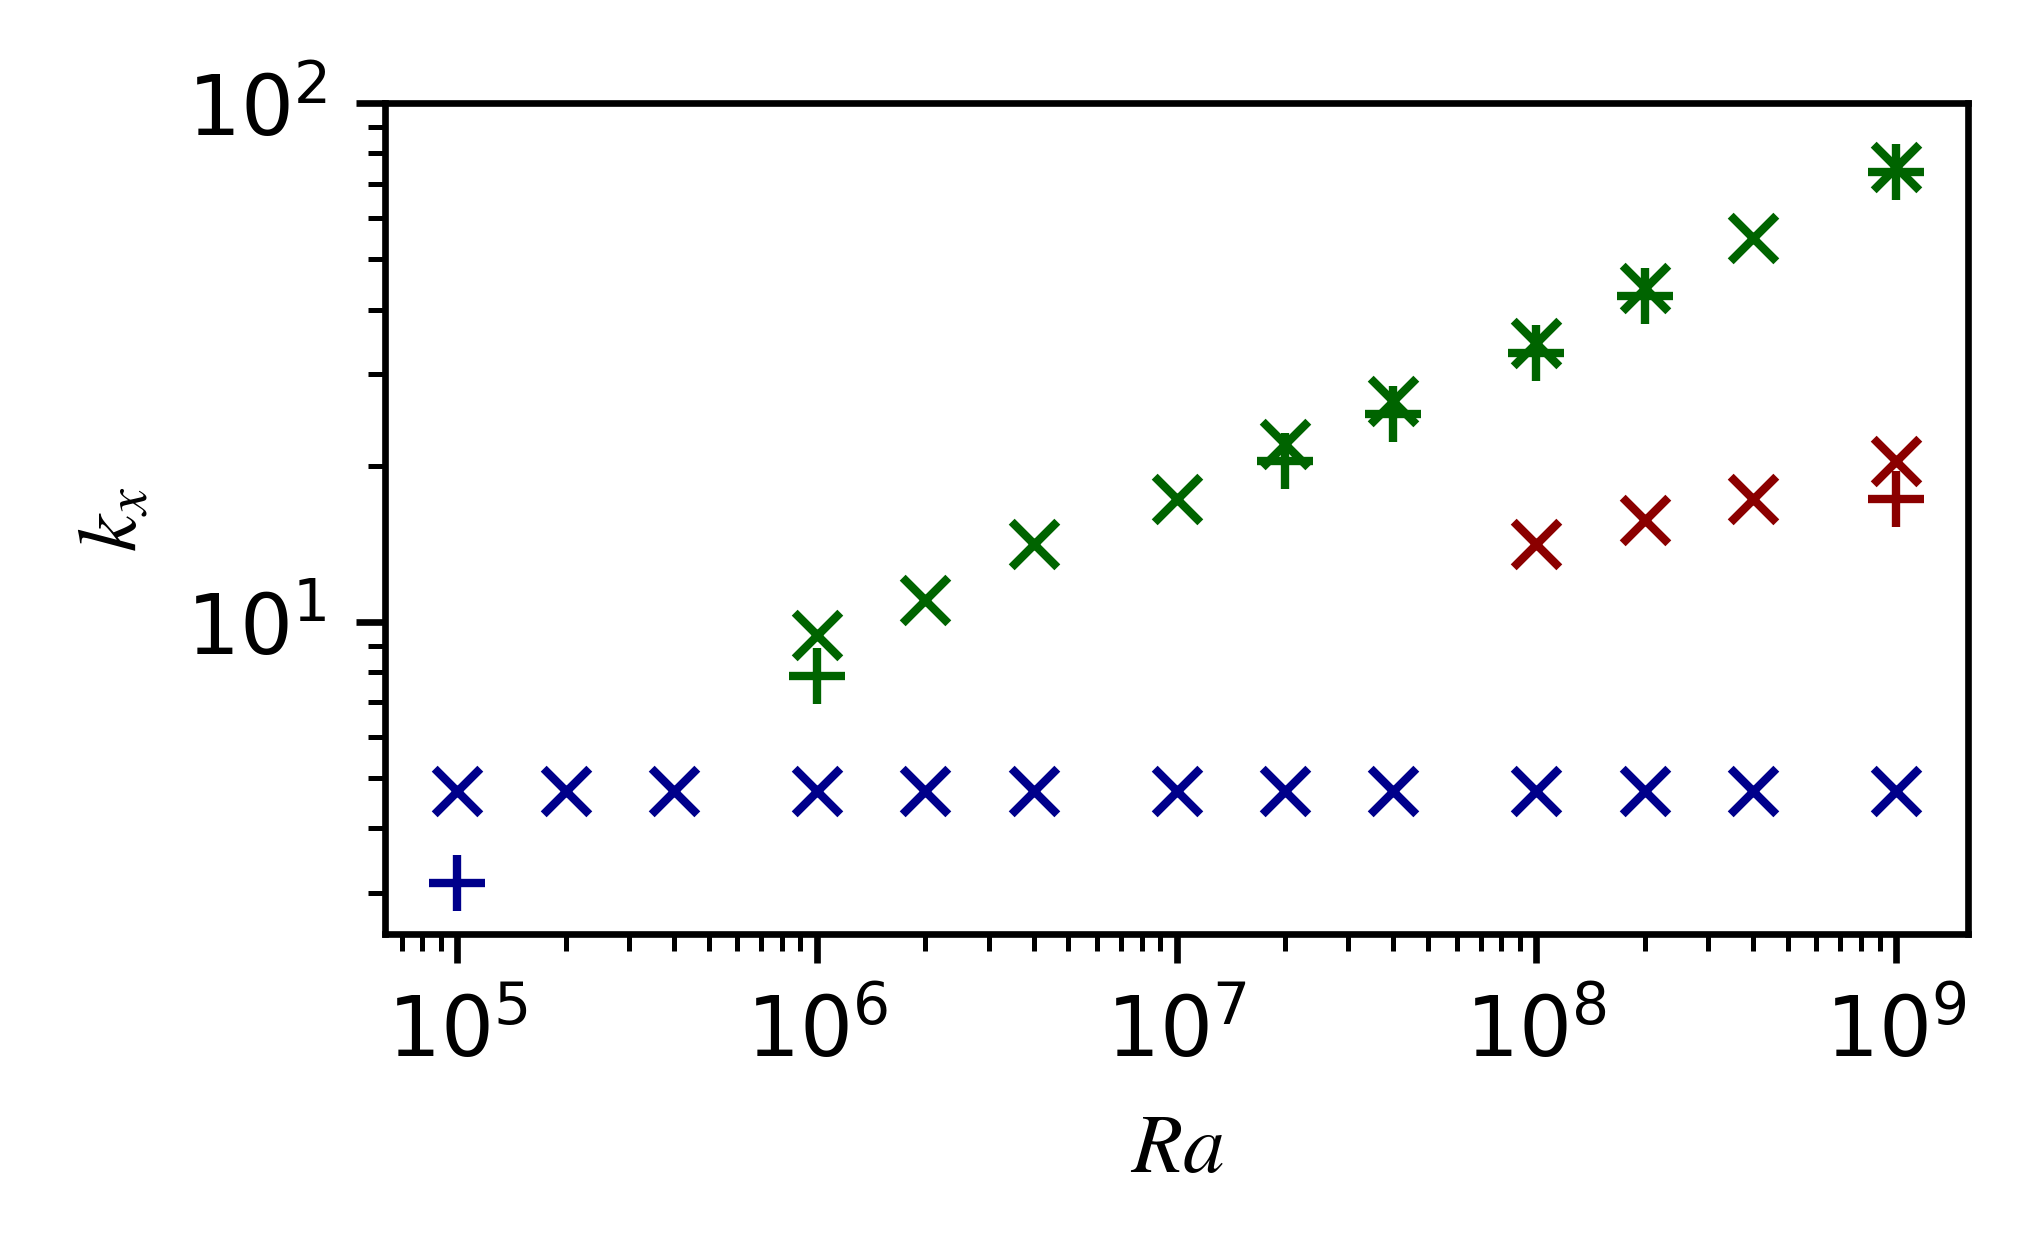
\includegraphics[width=3.4in]{kx_m_ra1.png}
    \caption{Wavenumbers of marginally-stable modes of thermally equilibrated states. 
    Markers are color-coded according to their adjacent local maxima index in the eigenvalue spectrum. 
    For example, the spectrum corresponding to $Ra = 10^5$ has adjacent marginal wavenumbers $k_x = \pi, \, 1.5\pi$. 
    The $Ra = 10^9$ spectrum, shown in lower right corner of Figure \ref{fig:flux}, has three groups of maxima, with a single marginal mode in the first group ($k_x = 1.5\pi$), two adjacent marginal modes in the second group ($k_x = 6\pi, \, 6.5\pi$), and two adjacent marginal modes in the third group ($k_x = 23.5\pi, \, 24\pi$). 
    The largest wavenumbers of the green branch obey a power-law relationship with $Ra$}
    \label{fig:kx_marginals}
\end{figure}

Thermally equilibrated states with large $Ra$ tend to have diverse combinations of marginal modes. 
In every case, the $k_x = 1.5\pi$ mode is included and is often unaccompanied by adjacent modes. 
In Figure \ref{fig:kx_marginals} we give the wavenumbers $k_x$ of marginal modes, color-coded according to their adjacencies. 
Marginal modes often appear in neighboring pairs, where the larger mode is denoted with an x and the smaller mode is denoted with a +. 
In these cases we infer the existence of a local maximum eigenvalue between the two adjacent marginally-stable modes. 
For $Ra \geq 10^6$, a second branch of marginal modes is introduced as shown in light green, obeying some power-law with respect to $Ra$. 
The introduction of this largest branch is likely required to oppose the diffusion of the thinning boundary layers. 
For $Ra \geq 10^8$, a third branch appears (shown in light blue), splitting the widening gap between the other branches. 
This development is associated with moderately thick advection profiles, filling a niche in the total flux by uniting the sharp profiles of the largest branch and those of the bulk-domain-oriented smallest branch.

\begin{figure}
    \centering
    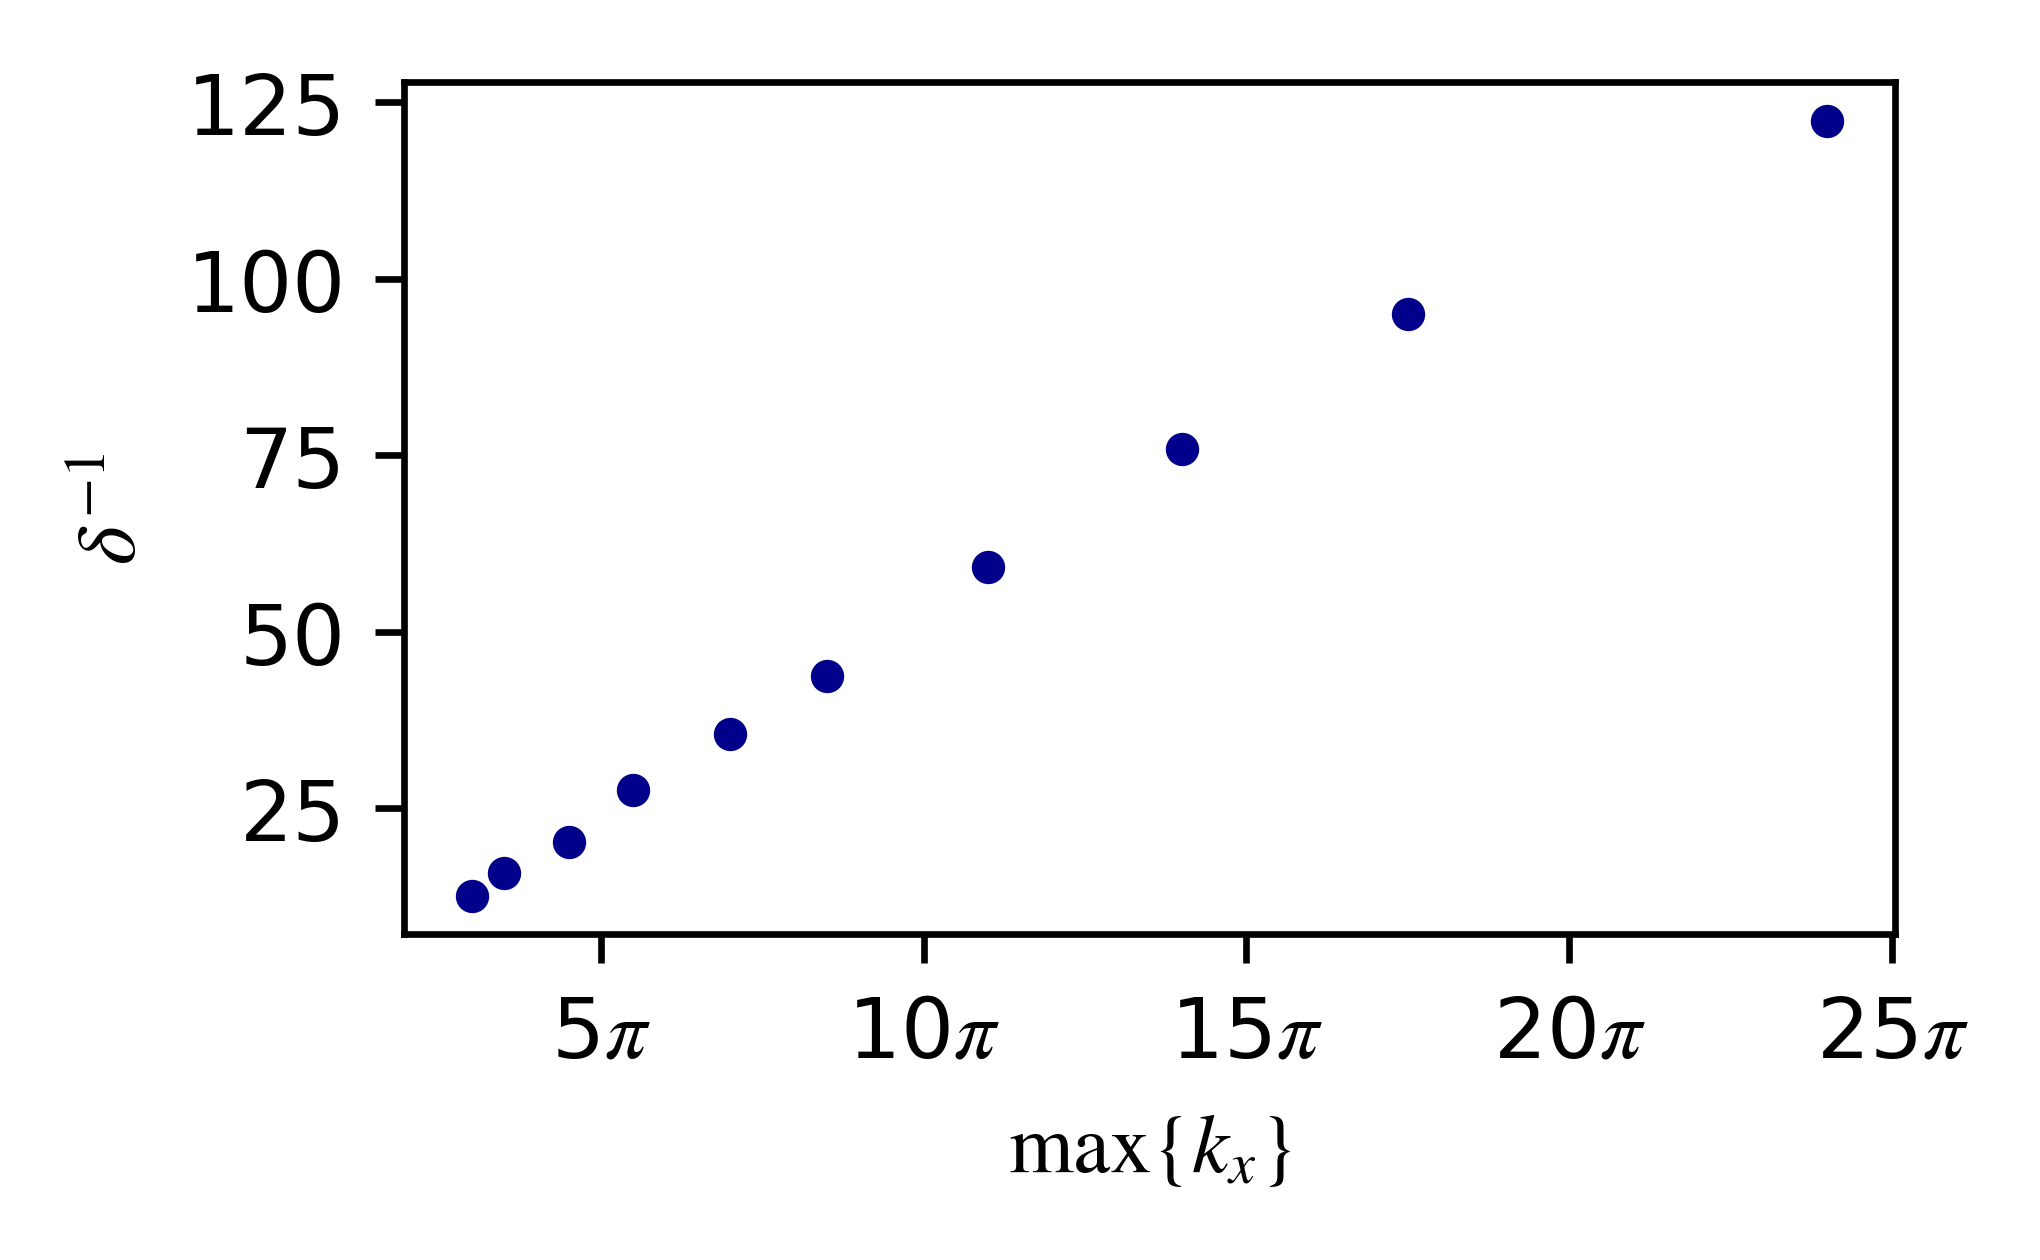
\includegraphics[width=3.4in]{del_kx_inv.png}
    \caption{For $Ra \geq 10^6$, the maximum marginally-stable wavenumbers (corresponding to the green X markers in Figure \ref{fig:kx_marginals}) are inversely related to the boundary layer heights $\delta$. 
    $(\max \{ k_x \})^{-1}$ gives a minimum $x$ length scale for the perturbations, and consequently, the advection. 
    We expect the minimum $z$ length scale to agree with the boundary layer height $\delta$ because otherwise the boundary layer would continue to diffuse. 
    This is illustrated in the lower left corner of Figure \ref{fig:flux}, where the advection profile for $k_x = 24\pi$ is tightly flanked by the surrounding boundary layer. 
    This suggests that the minimum $x$ and $z$ length scales obey some constant ratio over various $Ra$.}
    \label{fig:del_inv}
\end{figure}

The largest marginal wavenumber $\max \{ k_x \}$ (represented by the light green branch in Figure \ref{fig:kx_marginals}) serves as a inverse minimum length-scale in the $x$ direction. The finest structures in $\bar{T}(z)$ appear near the boundaries, providing us with a complementary minimum length-scale for $z$. We define the interior boundary layer threshold as the $z$-coordinate at which $\frac{\partial \bar{T}}{\partial z} = 0$. In Figure \ref{fig:del_inv}, we illustrate the constant ratio between these two quantities for various $Ra$. The quasilinear model cannot describe small-scale behaviors in either direction. Discretization of the normal modes allows us to collapse the problem into a single dimension, but this comes at a cost.  

\begin{figure}
    \centering
    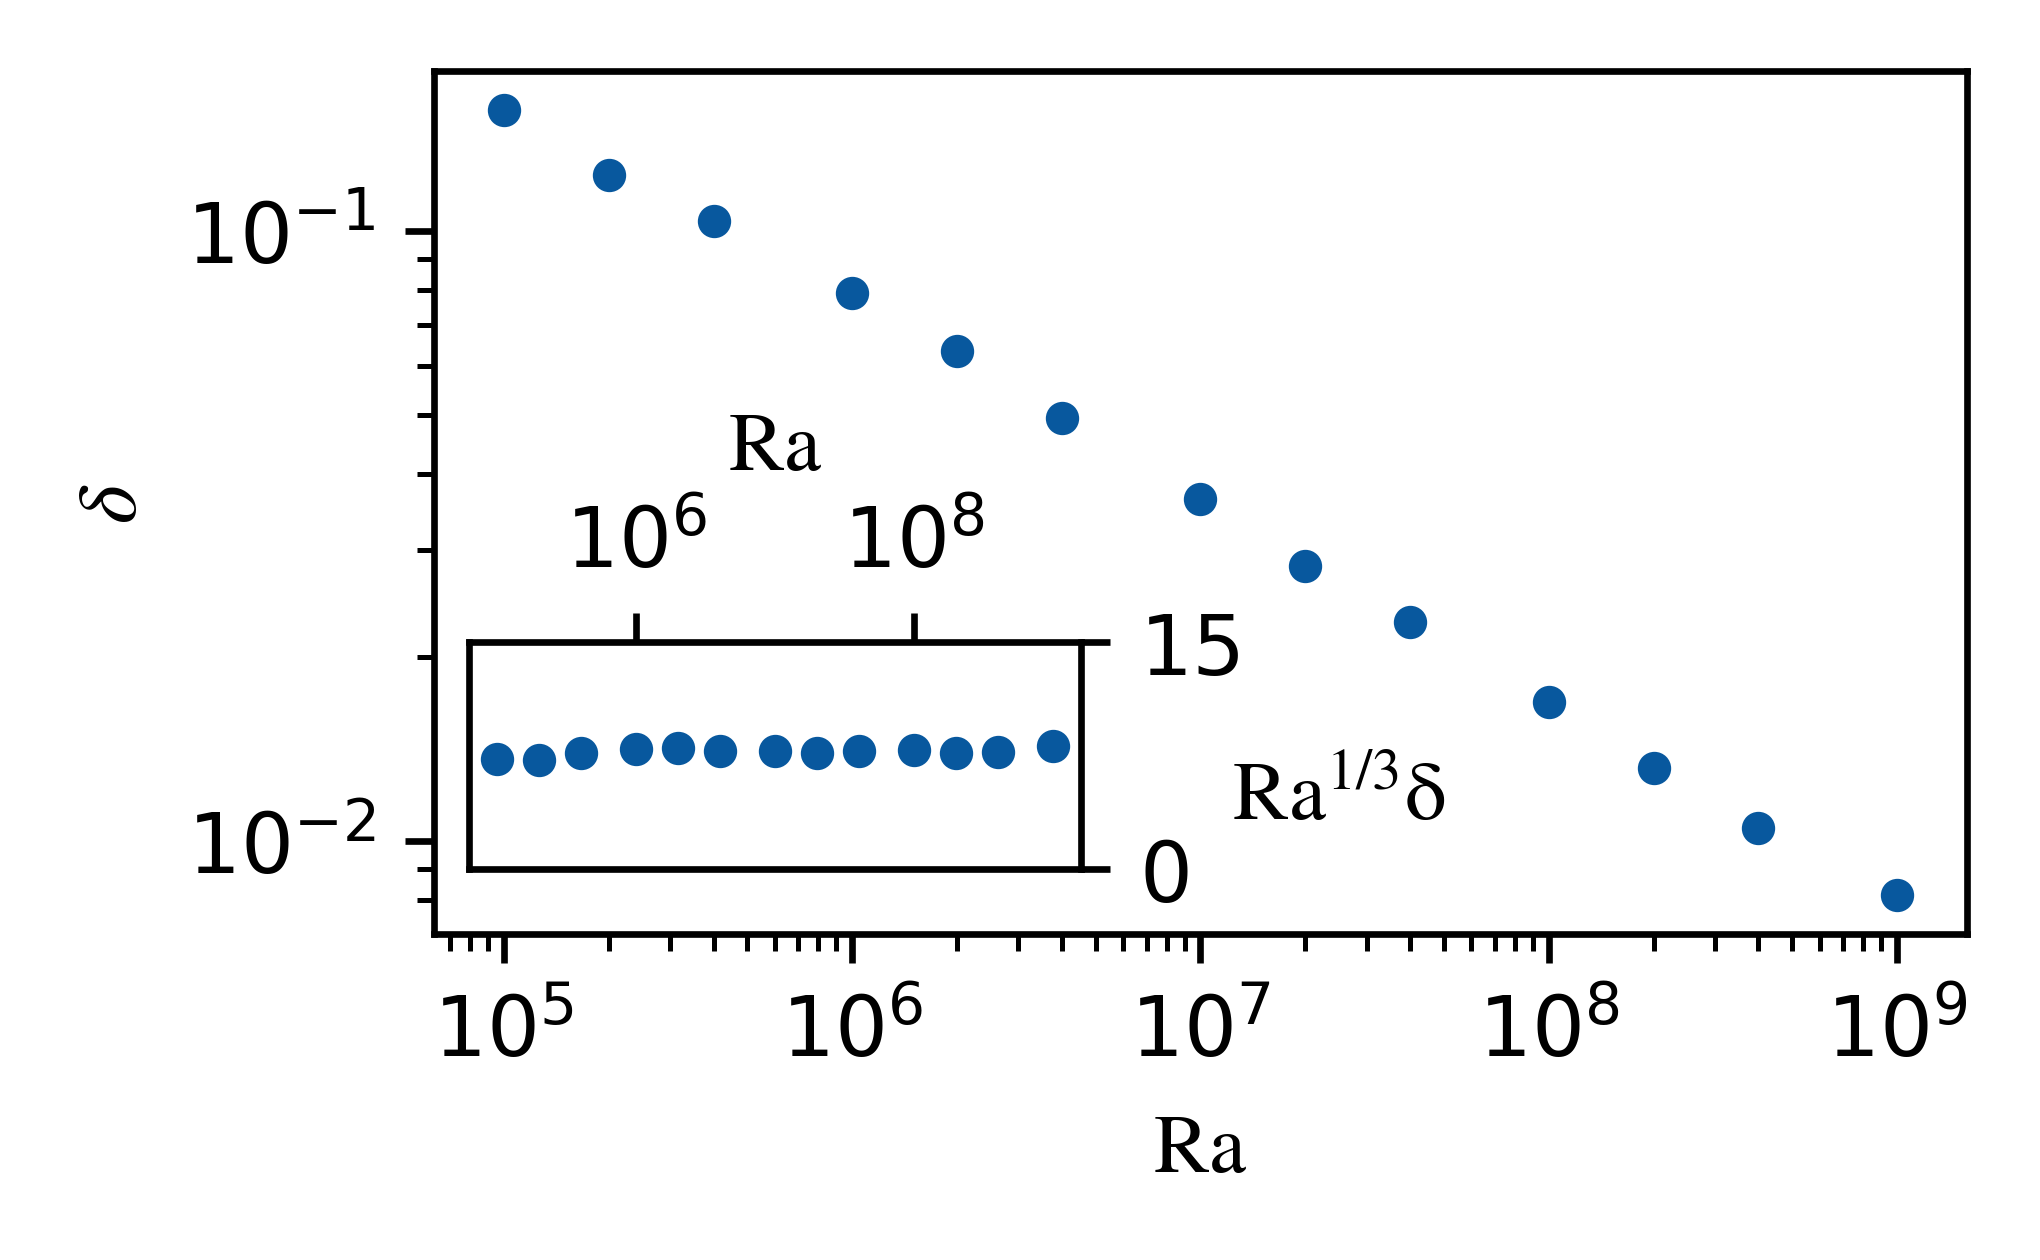
\includegraphics[width=3.4in]{del_ra.PNG}
    \caption{Boundary layer height $\delta$ of marginally-stable thermal equilibria. 
    We define the threshold of each boundary layer as the $z$-coordinate at which $\frac{\partial \bar{T}}{\partial z} = 0$, corresponding to the local extrema of the equilibrated curve in Figure \ref{fig:T0_profiles}. 
    Plotting on a log-log scale, we find that $\delta$ and $Ra$ obey a power-law relationship. We also demonstrate that $Ra^{1/3}\delta$ is approximately constant with respect to $Ra$ which is consistent with \cite{Malkus_1954, Wen}}
    \label{fig:bl_ra}
\end{figure}

In general, MSTE can be characterized by their boundary layer height, from which, the rest of their properties follow. In Figure \ref{fig:bl_ra}, we illustrate the scaling behavior of the boundary layer height $\delta = Ra^{-1/3}$. 
This is consistent with Malkus' classical marginal-stability theory, a scaling argument which perceives the boundary regions as subdomains which are themselves marginally-stable \cite{Malkus_1954}.

\begin{figure*}
    \centering
    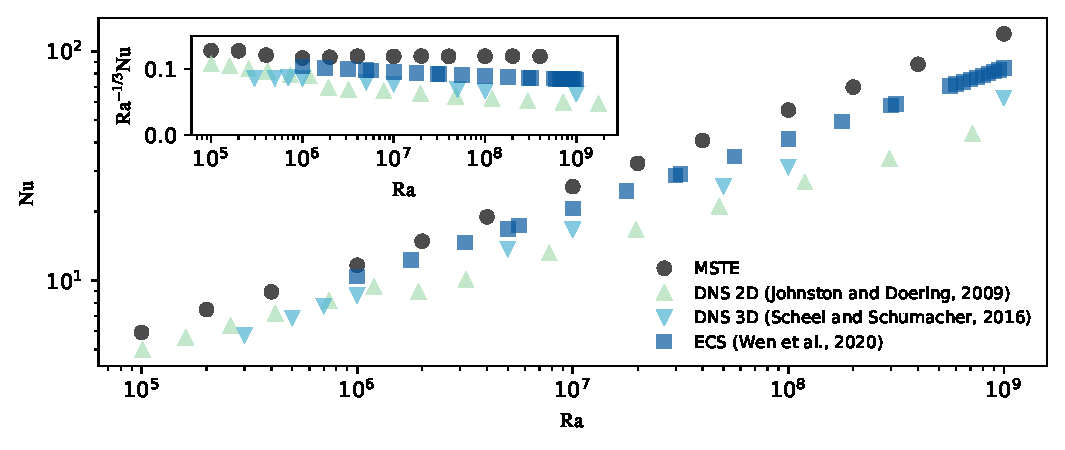
\includegraphics[width=7.1in]{nu_ra.PNG}
    \caption{Nusselt numbers are shown for MSTE, aspect-ratio-optimized ``steady rolls'' ECS \cite{Wen}, as well as statistically-steady 2D and 3D DNS \cite{Johnston, Scheel_2016}.
    All datasets obey power-law relationships, with the MSTE and ECS admitting classical scaling $\Nu \sim Ra^{1/3}$. 
    MSTE have greater $\Nu$ than the ECS, which in turn, have greater $\Nu$ than the DNS. This can be explained by the contrasting boundary layer geometries shown in Figure \ref{fig:T0_profiles}.}%
    \label{fig:nu_vs_ra}%
\end{figure*}

The Nusselt number, which measures convective performance, is given by
\begin{equation}
  \Nu = 1 + \frac{A^2}{\mathcal{P}} \langle w'T' \rangle_x.
\end{equation}
There is no general consensus surrounding the scaling behavior of $\Nu$ for high $Ra$ systems, which are of particular importance in astrophysical systems. In Figure \ref{fig:nu_vs_ra} we report $\Nu$ for MSTE, ``steady rolls" ECS \cite{Wen}, and DNS \cite{Scheel_2016, Johnston}. 
All states obey $\Nu \sim Ra^{\beta}$ with classical scaling $\beta = 1/3$ in the ECS and MSTE. 
\cite{Wen} hypothesized that $\Nu$ of ECS which admit classical Malkus scaling must always exceed $\Nu$ of turbulent convection.
If we generalize this notion to include quasilinear equilibria, our findings agree; MSTE have larger $\Nu$ than 2D and 3D DNS.
This might be due to the chaotic transitions, among the unstable periodic orbits outlined by \cite{Yalniz, Cvitanovic}, inhibiting heat flux. 
We might also anticipate the existence of similar equilibria, having smaller $\Nu$ and occupying complementary nodes in the Markov chain whose long-term behavior agrees with DNS. 

\section{Simulations with Thermally Equilibrated Initial Conditions}
This investigation is partially motivated by the prospect of decreasing DNS times by employing MSTE initial conditions. 
Conventionally, (\ref{EQ:motion1})--(\ref{EQ:motion3}) are solved via DNS with the linear initial conditions
\begin{align}
    T(x, z)\big|_{t=0} &= 0.5 - z \\
    \mathbf{u}(x, z)\big|_{t=0} &= \mathbf{0} \\
    p(x, z)\big|_{t=0} &= 0.
\end{align}
$t$ in this section now refers to the simulation time as opposed to the thermal equilibration time parameter used previously. 
We define the MSTE initial conditions
\begin{align}
    T(x, z)\big|_{t=0} &= \bar{T}(z) + \sqrt{2} \sum_{n=1}^N  A_n \text{ Re} \Big[ \theta_n(z) e^{ik_{x_n}x} \Big] \nonumber \\
    \mathbf{u}(x, z)\big|_{t=0} &= \sqrt{2} \sum_{n=1}^N A_n \text{ Re} \Big[\Big( U_n (z) \hat{x} + W_n(z) \hat{z} \Big) e^{ik_{x_n}x} \Big] \nonumber\\
    p(x, z)\big|_{t=0} &= \sqrt{2} \sum_{n=1}^N A_n \text{ Re} \Big[P_n (z) e^{ik_{x_n}x}\Big]
\end{align}
Where $\theta_n(z), U_n(z), W_n(z), P_n(z); \, A_n; $ and $k_{x_n}$ refer to the complex eigenfunctions, amplitude, and wavenumber at the $n$th marginal mode respectively. 
The $\sqrt{2}$ factor is necessary for eigenfunction normalization. 

Simulations with MSTE initial conditions do not exhibit a convective-transient period, as the large-scale anatomy of convective cells exists on initialization. 
This is illustrated in Figure \ref{fig:nu_sim}, where the sharp spike in $\Nu$ is associated with a turbulent transitional period of upwelling until the distinctive plume-like structure is established. 
Simulation of this transitional period is prohibitive \cite{Anders_AE}. 
For high $Ra$ experiments, researchers often ``bootstrap" data by initializing simulations with the results of similar $Ra$ runs \cite{Verzicco, Johnston}. 
MSTE can be perceived as a set of initial conditions, designed for avoiding the simulation of transitional high Reynolds number flows.

MSTE are laminar, lacking the small-scale structures associated with moderate to high $Ra$ experiments. 
The absence of chaotic dynamics is an apparent consequence of the quasilinear assumptions. 
If we treat MSTE as background states, DNS suggest that plumes, vortex sheets, and other unstable turbulent features inhibit total heat transfer. 
This perspective agrees with conventional models of transitions to turbulent flows, such as Boussinesq's turbulent-viscosity hypothesis \cite{boussinesq_1877}, where the emergence of small-scale velocity structures tends to increase total shear \cite{Lecoanet_KH, drazin_reid_2004, pope_2000}, thereby impeding buoyancy-driven flows and decreasing advection in the bulk of the domain. 
We could also attribute the diffuse DNS temperature profile in Figure \ref{fig:T0_profiles} with unsteady boundary-layer penetration and mixing that MSTE do not exhibit.

% \begin{figure}
%     \centering
%     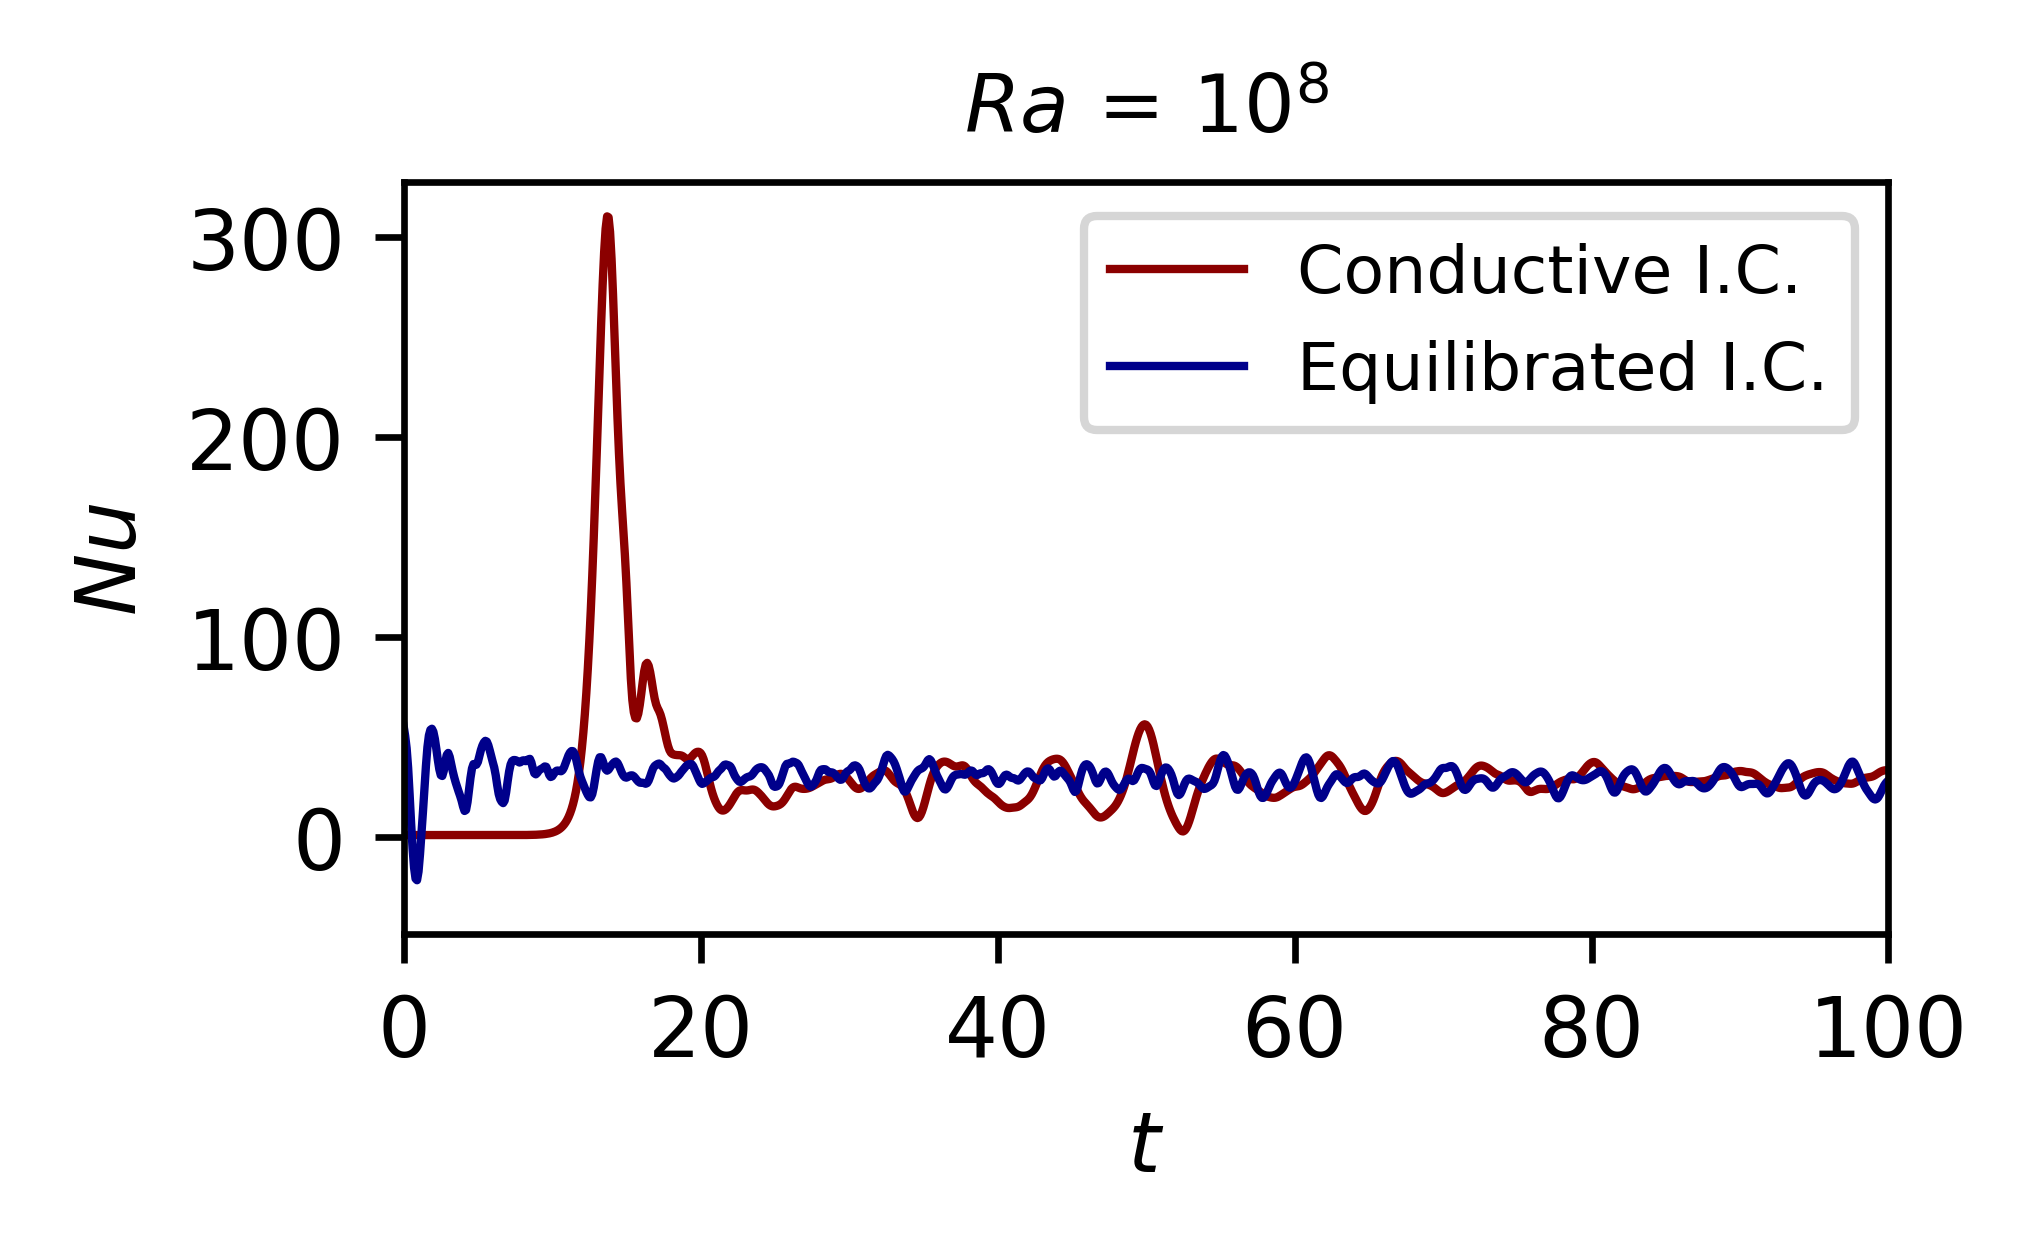
\includegraphics[width=3.4in]{sim_eq_nu.png}
%     \caption{Nusselt numbers of simulations performed at $Ra \, = \, 10^8$ with conventional initial conditions (red) and marginally-stable thermally-equilibrated initial conditions (blue). Simulations launched with thermally-equilibrated states do not undergo a convective-transient period because the characteristic plume structure exists on initialization. This is illustrated by the $Nu$ spike at $t \sim 15$ in the convectional simulation.}
%     \label{fig:nu_sim}
% \end{figure}
The average kinetic energy MSTE is significantly larger than the statistical steady state, as shown Figure \ref{fig:ke_sim}. 
This is postpones kinetic relaxation because the large-scale flows decay on a viscous time-scale
\begin{equation}
    t_{\nu} \sim \sqrt{\frac{Ra}{Pr}}. \nonumber
\end{equation}
Consequently, MSTE initial conditions do not reduce the simulation time required to achieve a statistically steady state -- instead they increase it considerably. This suggests the MSTE background state perspective is partially flawed, as an appropriate background state would approximate $\langle|\mathbf{u}|^2 \rangle_{\mathcal{D}}$ with more fidelity.
% \begin{figure}
%     \centering
%     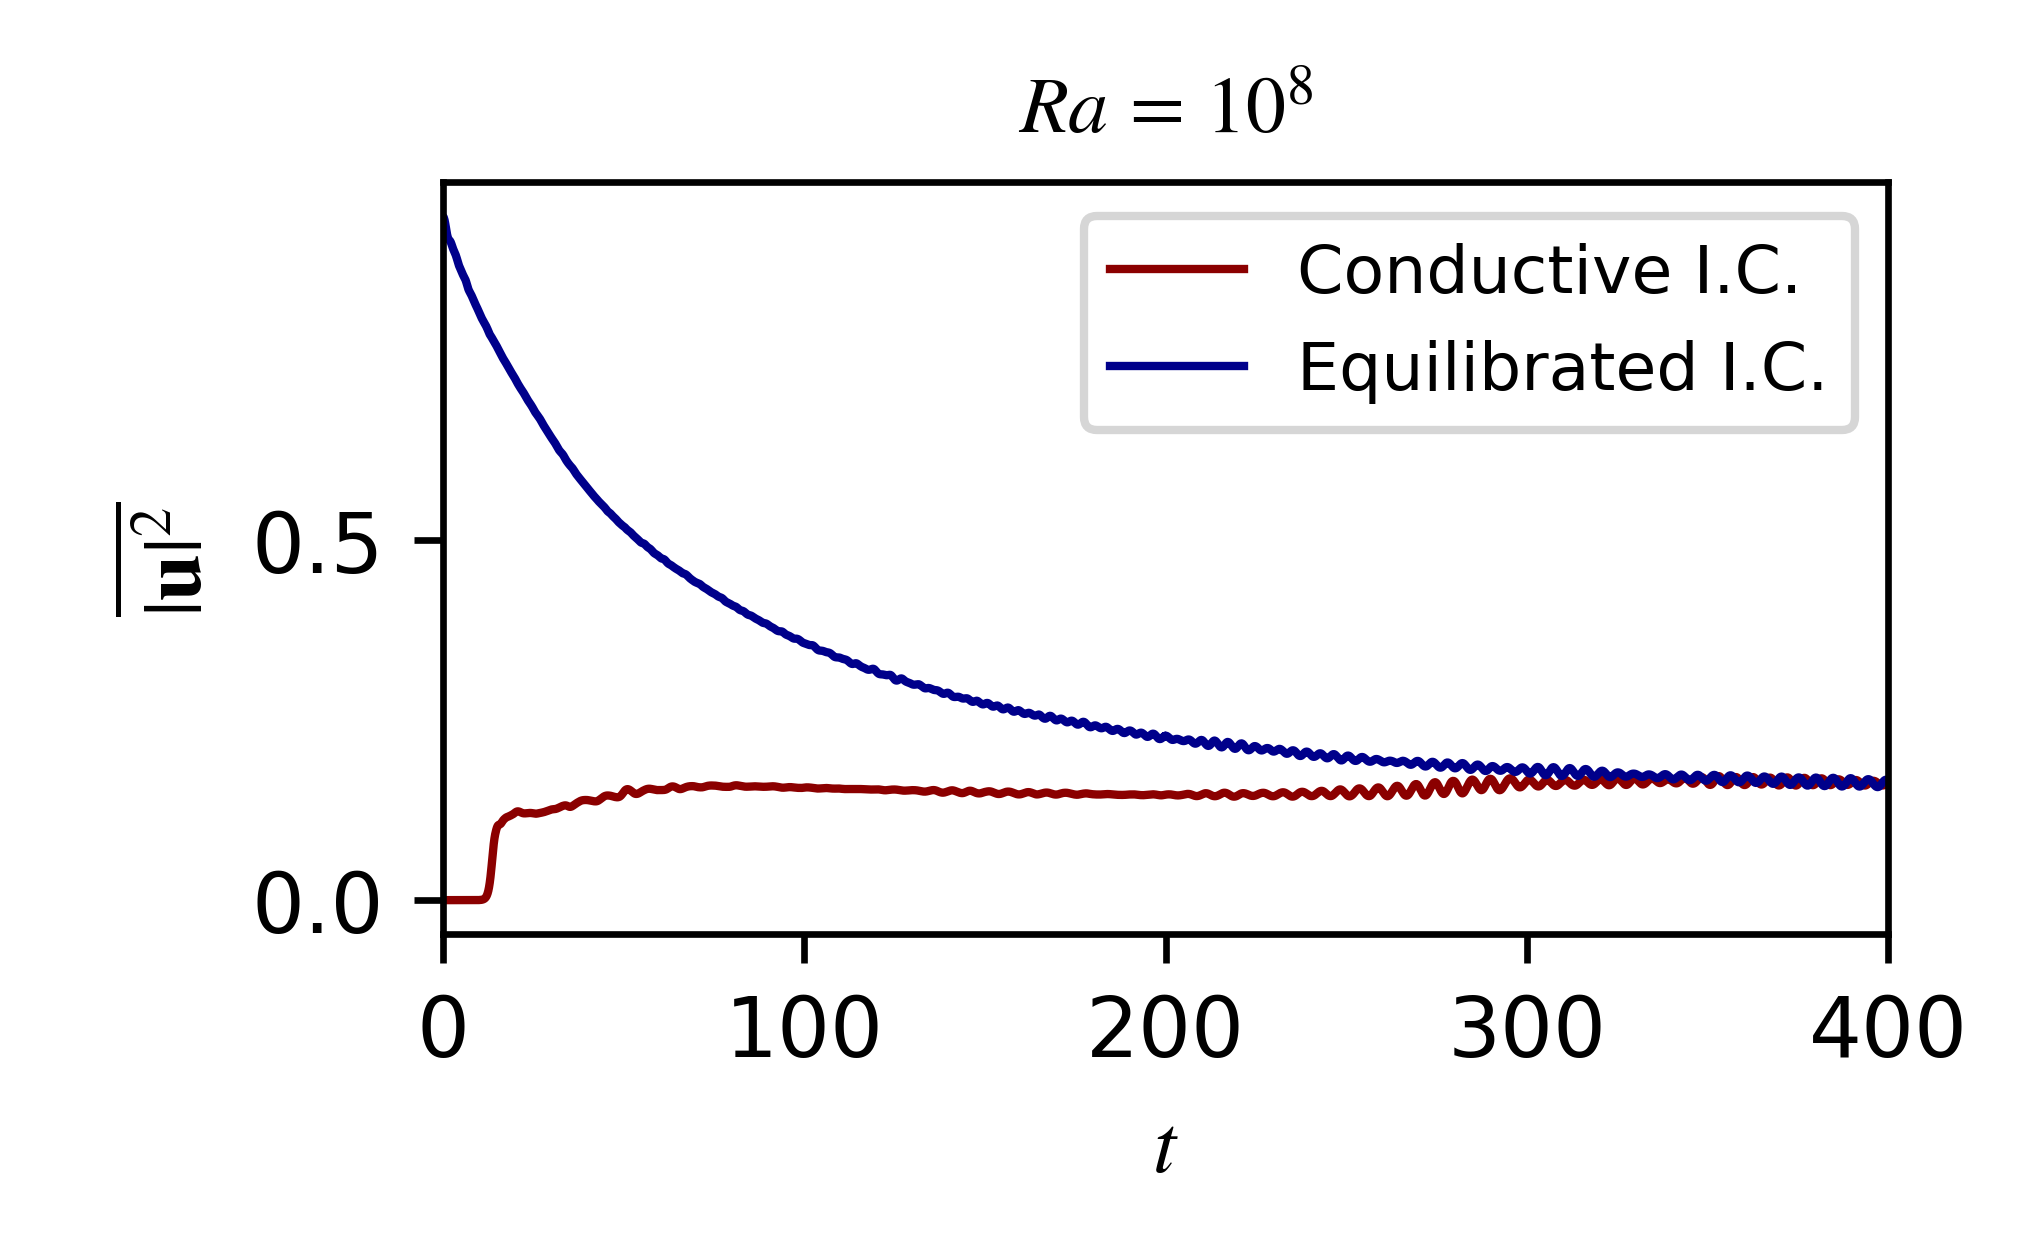
\includegraphics[width=3.4in]{sim_eq_ke.png}
%     \caption{Average kinetic energies of the same simulations performed in Figure \ref{fig:nu_sim} ($Ra = 10^8$). The combination of eigenfunctions which give thermal equilibrium have significantly more kinetic energy than the statistically steady state. Kinetic equilibrium is achieved according to the viscous timescale $t_{\nu} \sim Pr Ra^{-1/2}$.}
%     \label{fig:ke_sim}
% \end{figure}
\begin{figure}
    \begin{minipage}{3.4in}
        \centering
        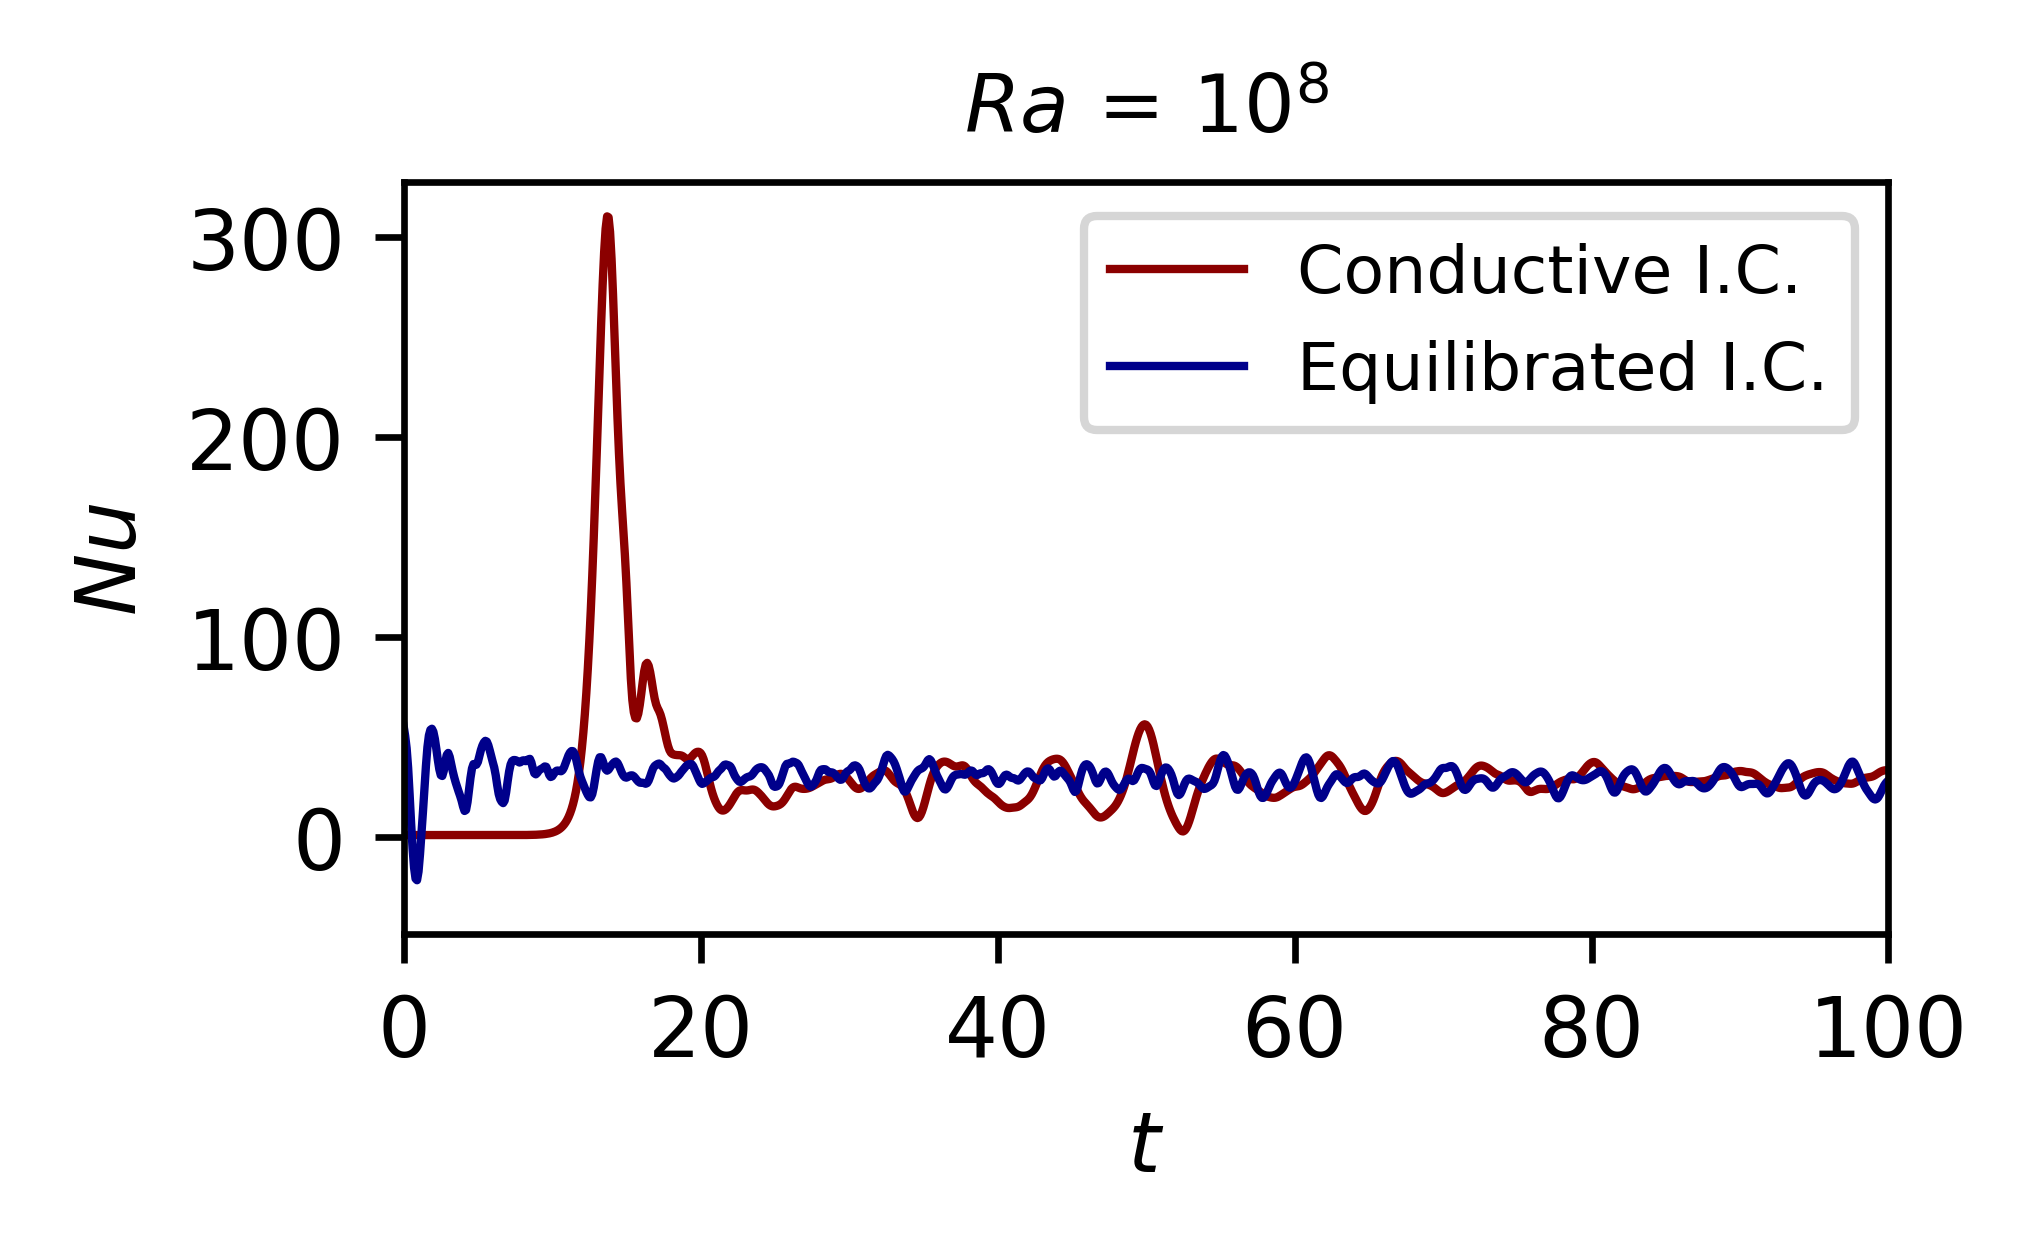
\includegraphics[width=3.4in]{sim_eq_nu.png}
        \caption{Nusselt numbers of simulations performed at $Ra = 10^8$ with the conventional initial conditions (black) and MSTE initial conditions (blue). 
        MSTE simulations do not undergo a convective-transient period because the characteristic large-scale convective cell structure exists on initialization.}
        \label{fig:nu_sim}
    \end{minipage}
\end{figure}

\begin{figure}
    \begin{minipage}{3.4in}
        \centering
        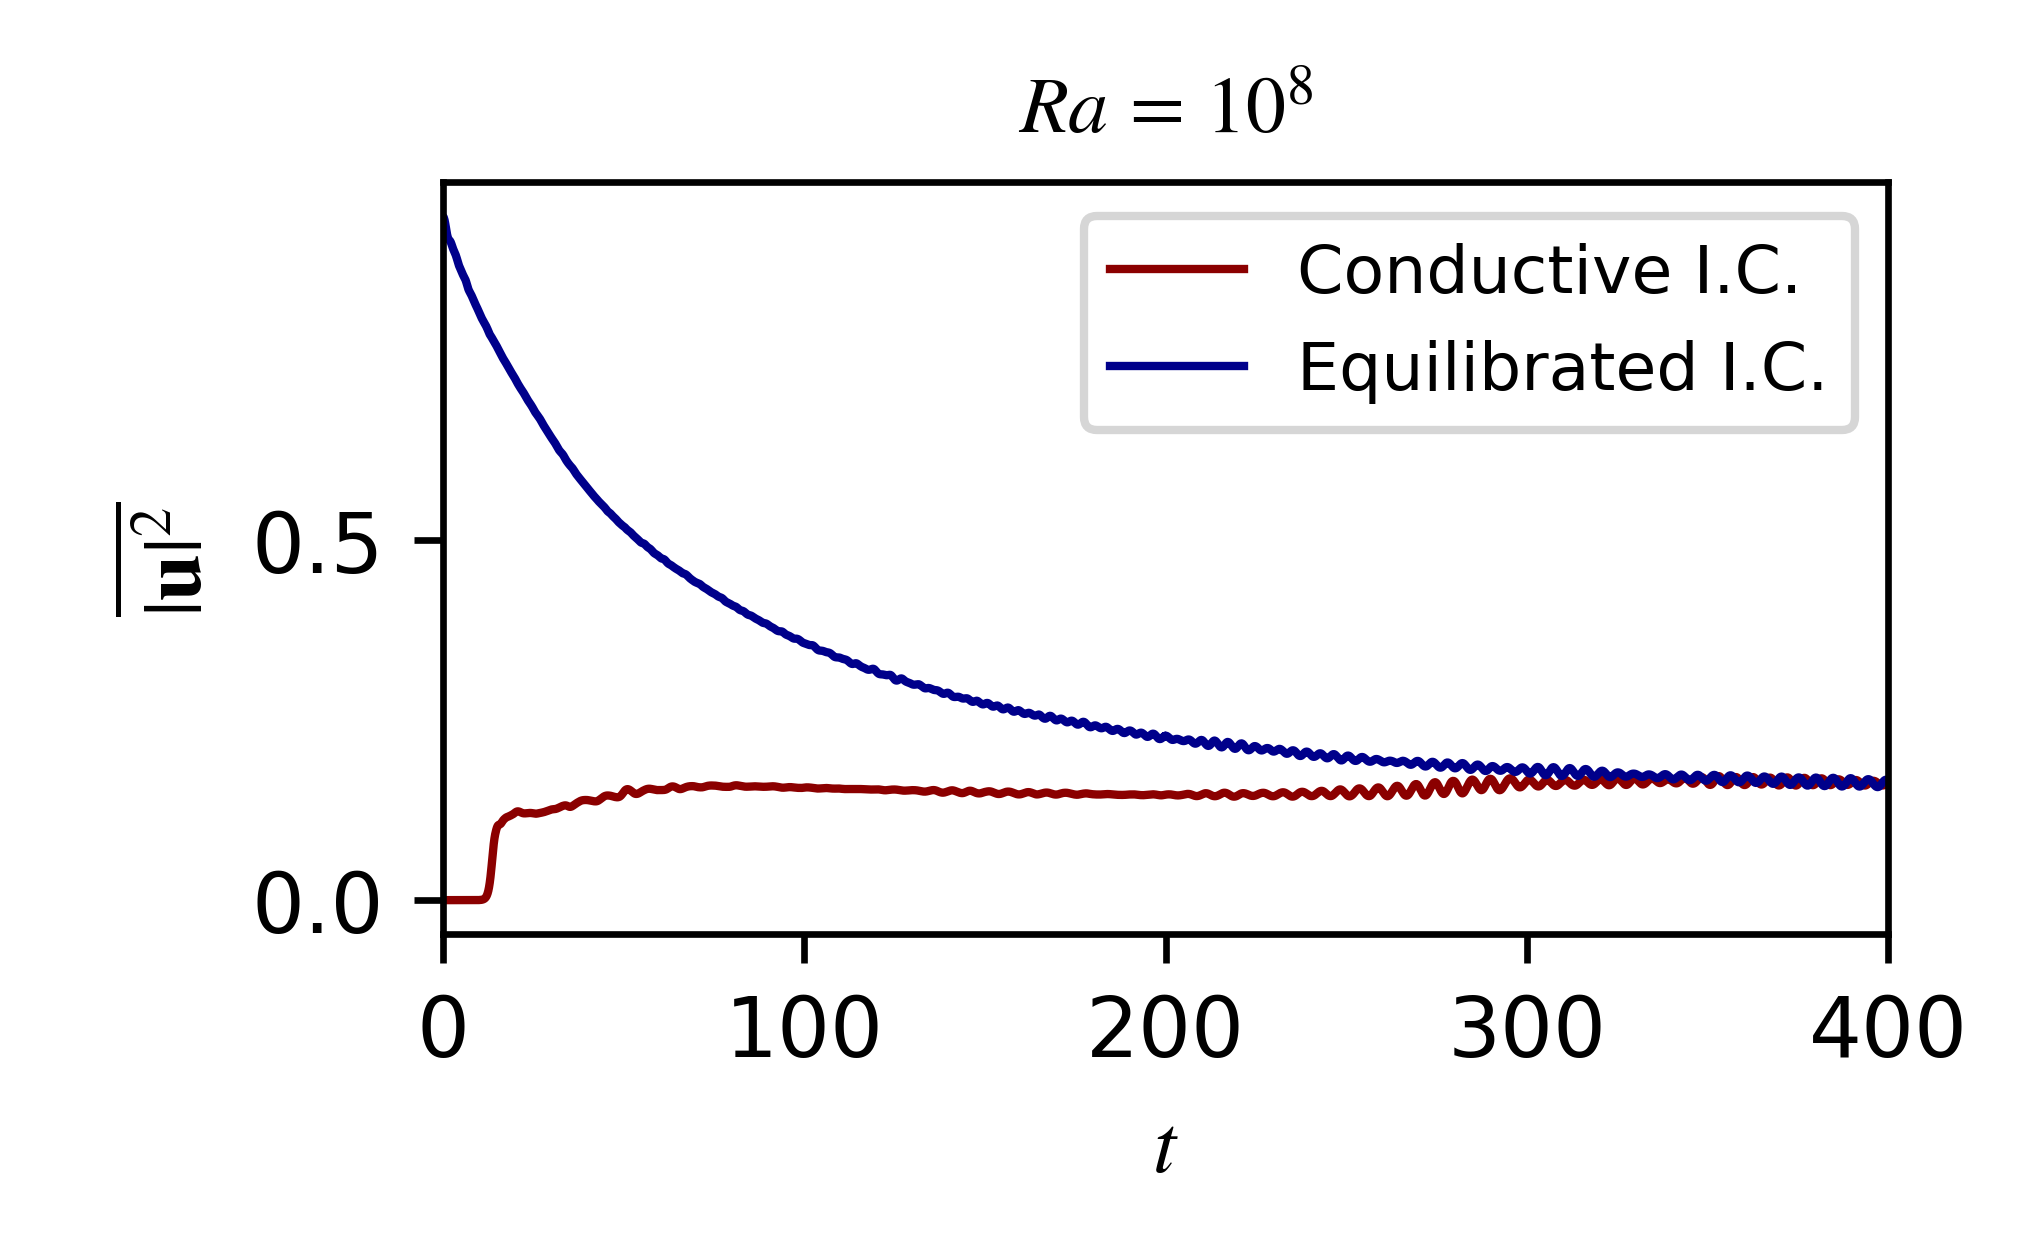
\includegraphics[width=3.4in]{sim_eq_ke.png}
        \caption{Average kinetic energies are reported for the simulations performed in Figure \ref{fig:nu_sim} at $Ra = 10^8$. 
        The combination of eigenfunctions associated with MSTE have significantly more kinetic energy than the statistically steady state. 
        Kinetic equilibrium is achieved according to the viscous timescale $t_{\nu} \sim \sqrt{Ra / Pr}$.}
        \label{fig:ke_sim}
    \end{minipage}
\end{figure}

\section{Discussion}\label{sec:Discussion}
In general, the reduced model we study in this paper can be perceived as a unique way to describe Rayleigh–Bénard convection. 
To compute MSTE, we construct a marginally-stable mean temperature profile and develop the quasilinear model via independent time-scales.
Solutions retain several key features that are ubiquitous in experiments and simulations: $\Nu \sim Ra^{1/3}$ scaling, large-scale convective cell structures, and agreement with classical minimum length-scale approximations \cite{Malkus_1954}. 
They also exhibit unique and unexpected features: mean temperature gradient-reversals/dips, kinetic exaggeration, and greater $\Nu$ than other time-invariant solutions. 
We obtain indistinguishable solutions despite initializing with various mean temperature profiles $\bar{T}(z, 0)$. 
Thus solutions might be unique, but we cannot demonstrate this rigorously.

% Simulations performed with MSTE initial conditions do not undergo an initial convective transient period, 

As previously noted, solving the EVP for statistically steady DNS data yields positive eigenvalues; the system is in a perpetual state of instability. 
Unstable modes tend to stabilize the system rapidly, creating a negative feedback loop whose average state is linearly unstable. 
We might curtail the disagreement between MSTE and DNS by loosening our marginal-stability criterion. 
Should the time-scales not be entirely separate, we might anticipate the long-term persistance of moderately unstable modes. 
This perpetual instability cannot be described by our model independently (we do not know, a priori, how unstable such modes are) but it might prove fruitful to investigate moderately unstable thermal equilibria (MUTE). 
More precisely, instead of traversing the manifold of marginally-stable states toward MSTE, we could consider the manifold of states whose maximum eigenvalue(s) $\omega_{\rm{max}}$ agree with some other stability constraint. 
Note that under this definition, 2-dimensional ECS are themselves MUTE, because they are thermally-equilibrated and generally unstable, though they need not satisfy the quasilinear form.

We cannot use our reduced quasilinear model to predict $\Nu \sim Ra^{\beta}$ for large $Ra$ without some complementary stability constraint. 
The eigenvalues of DNS data might provide an informative stability constraint (we could find MUTE and compare them with DNS data), but this would be self-defeating in general. 
Instead we seek to combine reduced models to approximate $\beta$ without DNS. Under the marginal-stability constraint, we found that MSTE exhibit classical Malkus scaling, having marginally-stable boundary layers with $\beta = 1/3$. 
We could instead require that the eigenvalues of MUTE agree with the eigenvalues of the analytic 1-dimensional boundary layer predictions of \cite{Shishkina, Zhang_20} (which remain in development), allowing us to refine and expand these estimates into 2-dimensional MUTE. 
Accessible MUTE states would not rely on DNS, satisfying only the quasilinear problem and stability constraint. 
Such MUTE ought to agree with DNS data more precisely than MSTE, ideally having slower flows. 
This is reasonable to expect, since accurate boundary layer approximations and DNS data should have similar stability characteristics. 
By definition, MUTE are unstable and would therefore admit more diffuse boundary layer structures, requiring smaller $A^2(t)$ (less advection) to satisfy the stability constraint and thereby reducing $\Nu$, $\langle |\mathbf{u}|^2 \rangle_{\mathcal{D}}$ and possibly $\beta$.

\section*{Appendix}
\subsection{Initial buoyancy profile} \label{sec:initial_profile}
We initialize the thermal-equilibration algorithm with \cite{Shishkina}'s analytical thermal boundary layer equation for turbulent Rayleigh-B\'enard convection, given by 
\begin{align}
    \bar{T}_0(\xi) &= \frac{\sqrt{3}}{4\pi} \log \frac{(1 + a\xi)^3}{1 + (a\xi)^3} + \frac{3}{2\pi} \arctan \Big( \frac{4\pi}{9}\xi - \frac{1}{\sqrt{3}} \Big) + \frac{1}{4} \nonumber \\
    \xi &= \frac{z}{\delta_0}, \qquad a = \frac{2\pi}{3\sqrt{3}}\label{EQ:T0}
\end{align}
where $\delta_0$ is the boundary layer height. 
We expect that each $\Ra$ is associated with a unique $\delta_0$ for which $\bar{T}_0(z)$ is marginally-stable. 
It should be noted that when experimenting with various initial profiles $(\tanh, \rm{erf}, \rm{etc.})$, we obtain indistinguishable equilibrated states, implying that solutions may be unique. 
An example of (\ref{EQ:T0}) is given by the blue curve in Figure \ref{fig:T0_profiles}.

\section*{Acknowledgments}
The authors thank Jeff Vassil, Greg Chini, Emma Kaufman for their valuable feedback and suggestions. 
We also thank the \texttt{Dedalus} and \texttt{Eigentools} development teams. 
Computations were performed on the NASA Pleiades system.


% \bibliographystyle{plain}
\bibliography{he}

\end{document}